\chapter{Horocyclic Groups}\label{chap1}

\section{The Poincar\'e Model of the Hyperbolic Plane}\label{chap1:sec1}\pageoriginale

Let $\mathfrak{H}$ denote the upper half-plane \{$\tau=x+iy, x, y$
real and $y>0$\}. It is well-known that any conformal mapping of
$\mathfrak{H}$ onto itself is given by
\begin{equation*}
\tau \to \tau^{\ast} = x^{\ast} + iy^{\ast} = S<\tau > =
\frac{a\tau+b}{c\tau+d}, \tag{1}\label{eq1:1}
\end{equation*}
where $S=\left(\begin{smallmatrix} a&b\\c&d\end{smallmatrix}\right)$
  is a matrix with $a, b, c, d$ real and determinant $|S|$ equal to
  1. All such matrices form a group under matrix multiplication and we
  denote this group by $\Omega$. For $S_1, S_2$ in $\Omega$, we
  clearly have $(S_1S_2)<\tau> = S_1 < S_2 <\tau>>$. It is obvious
  that two elements $S_1$ and $S_2$ of $\Omega$ define the same
  mapping of $\mathfrak{H}$ if and only if $S_1 =\pm S_2$. The domain
  $\mathfrak{H}$ together with $\Omega$ can be looked upon as a model
  for the hyperbolic plane. \textit{The hyperbolic straight lines} in
  this plane are defined by the segments of the circles (Here and in
  the following, circles include straight lines) orthogonal to the
  real axis, which lie in the upper half-plane. On $\mathfrak{H}$, we
  have a metric form
\begin{equation*}
ds^2 = \frac{d\tau d\bar{\tau}}{y^2} = 
\frac{dx^2+dy^2}{y^2}. \tag{2}\label{eq1:2}
\end{equation*}

Since 
\begin{equation*}
d\tau^{\ast} = (c\tau + d)^{-2} d \tau \quad \text{and} \quad y^{\ast}
= |c\tau+d|^{-2} y, \tag{3}\label{eq1:3}
\end{equation*}
the metric form \eqref{eq1:2} is left invariant by the transformations of
$\Omega$. We shall show that with respect to this metric form, the
hyperbolic straight line joining any two points of $\mathfrak{H}$ is
the path of shortest distance joining the two points. It is sufficient
to prove this assertion for the points $i$ and $iy_0(y_0 \geq
1)$, \pageoriginale since for any two points $\tau_1$ and $\tau_2$ in
$\mathfrak{H}$, there exists an element $S\in \Omega$ mapping
$\tau_1, \tau_2$ respectively to $i$ and $iy_0$ (with a suitable
$y_0\geq 1$) and further any transformation from $\Omega$ maps
hyperbolic straight lines to hyperbolic straight lines, leaving the
metric form invariant. Let $\tau=\tau(t) = x(t) + iy (t)$ for $a\leq t
\leq b$ be a parametric representation of a continuously
differentiable curve joining $i$ and $iy_0$. Then
\begin{equation*}
s = \int^b_a \frac{\sqrt{\dot{x}(t)^2 + \dot{y}(t)^2}}{y(t)} dt \geq
\int^b_a \frac{|\dot{y}(t)|}{y(t)} dt \geq \left|\int^b_a
\frac{\dot{y}(t)}{y(t)}dt\right| . \tag{4}\label{eq1:4}
\end{equation*}

It $\tau(t)$ were a curve of minimum length, equality must hold
everywhere in \eqref{eq1:4}, because, otherwise, the curve $\tau=iy(t)$ for
$a\leq t \leq b$, which also joins $i$ and $iy_0$ would be of shorter
length; or the given curve $\tau=\tau(t)$ would contain at least one
double point, but this is impossible. This shows, because of the
continuity of $\dot{x}(t)$, that $\dot{x}(t)$ and therefore $x(t)$
also vanishes identically and finally that $y(t)$ is monotonically
increasing. Thus the curve of minimal length between $i$ and $iy_0$
must be the hyperbolic straight line joining them, therefore we can
choose $t=y$ as a parameter and obtain
\begin{equation*}
s = \int^b_a \frac{\dot{y}(t)}{y(t)} dt = \int^{y_0}_1 \frac{dy}{y} =
log y_0 = \log ((i, iy_0, 0, \infty)), \tag{5}\label{eq1:5}
\end{equation*}
where $(z_1, z_2, z_3, z_4)$ generally denotes the cross ratio of the
four points $z_1, z_2, z_3$ and $z_4$ in the extended complex plane
defined by $(z_1, z_2, z_3, z_4)=
\dfrac{(z_2-z_3)(z_1-z_4)}{(z_1-z_3)(z_2-z_4)}$. If one of the four
points say $z_4=\infty$, we take $\dfrac{z_1-z_4}{z_2-z_4}\break =1$. Hence,
for any two points $\tau_1$ and $\tau_2$ of $\mathfrak{H}$, we obtain
from \eqref{eq1:5} \pageoriginale the following formula for the shortest distance:
\begin{equation*}
s = \log ((\tau_1, \tau_2, \sigma_1, \sigma_2)) = \rho(\tau_1,
\tau_2), \tag{6}\label{eq1:6}
\end{equation*}

\begin{figure}[H]
\centering
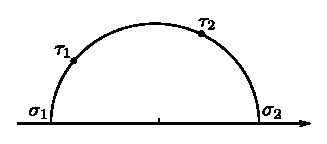
\includegraphics{vol29-fig/fig29-1.eps}
\smallskip
\caption{}
\label{chap1:fig1}
\end{figure}

with $\sigma_1, \sigma_2$ representing the points of intersection of
the hyperbolic line joining $\tau_1, \tau_2$ and the real axis. It can
be proved easily that $\mathfrak{H}$ provided with the distance
formula \eqref{eq1:6} is a metric space and this metric on $\mathfrak{H}$ is
left invariant by elements of $\Omega$. Moreover, it is well known
that this metric defines on $\mathfrak{H}$ the same topology as the
usual topology i.e. the topology induced from complex numbers. On
$\mathfrak{H}$, we have the measure
\begin{equation*}
d\omega = \frac{dx dy}{y^2}, \tag{7}\label{eq1:7}
\end{equation*}
which is invariant under transformations of $\Omega$ in view of the
formula
$$
\frac{\partial(x^{\ast}, y^{\ast})}{\partial(x,y)} =
\left|\frac{d\tau^{\ast}}{d\tau}\right|^2 = y^{\ast^2} /y^2.
$$

We shall prove that the area $\mathfrak{I}(A,B,C)$ with respect to the
measure in \eqref{eq1:7} of a hyperbolic triangle $(A,B,C)$ i.e. a triangle with
hyperbolic straight lines as edges with $\alpha, \beta$ and $\gamma$
as angles (see figure~\ref{chap1:fig2} is $\pi-\alpha-\beta-\gamma$. In order to
find $\mathfrak{I}(A,B,C)$ it is sufficient to find the area of the
triangles $(A,B,\infty)$, $(A,C,\infty)$ and $(B,C,\infty)$, because 

\begin{figure}[H]
\centering
\includegraphics{vol29-fig/fig29-2.eps}
\bigskip
\caption{}
\label{chap1:fig2}
\end{figure}

$\mathfrak{I} (A,B,C)=\mathfrak{I}(A,B,\infty) - \mathfrak{I}(A,C,\infty)
- \mathfrak{I}(B,C,\infty)$. If $(A,B,\infty)$ is a hyperbolic
triangle,\pageoriginale with the angles $\alpha, \beta$ and $0$ (see
figure~\ref{chap1:fig3}, then 
$\mathfrak{I}(A,B,\infty)=\pi-\alpha-\beta$; indeed,

\begin{figure}[H]
\centering
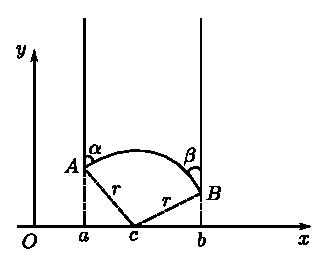
\includegraphics{vol29-fig/fig29-3.eps}
\smallskip
\caption{}
\label{chap1:fig3}
\end{figure}

\begin{align*}
\mathfrak{I}(A,B,\infty) &
=\iint\limits_{A,B,\infty}\dfrac{dxdy}{y^2} \\
& = \int\limits^b_a dx \int\limits^{\infty}_{\sqrt{r^2-(x-c)}} y^{-2}
dy\\
& = \int\limits^b_a \frac{dx}{\sqrt{r^2-(x-c)^2}} = \text{arc} \sin
\left(\frac{b-c}{r}\right)-\text{arc} \sin \left(\frac{a-c}{r}\right)\\
& = \left(\frac{\pi}{2}-\beta\right) - \left(\alpha -
\frac{\pi}{2}\right) = \pi - \alpha - \beta. 
\end{align*}

Let $\mathfrak{L}$ denote the unit disc \{$z=u+iv,u,v$ real and
$|z|<1$\}. The mapping 
$$
\tau \to z = \frac{\tau-i}{\tau + i} = A <\tau> \text{with} A =
\left(\begin{smallmatrix}
1&-i\\1&i\end{smallmatrix}\right)
$$
maps $\mathfrak{H}$ conformally onto $\mathfrak{L}$. If $\tau^{\ast} =
S<\tau>$ is mapped to $z^{\ast}$ in $\mathfrak{L}$, then 
$$
z^{\ast} = A <\tau>^{\ast} = A S <\tau> = A S A^{-1} <z> = L <z>,
$$
with $L = ASA^{-1} =\left(\begin{smallmatrix}
1&-i\\1&i\end{smallmatrix}\right)\left(\begin{smallmatrix}
a&b\\c & d\end{smallmatrix}\right)\left(\begin{smallmatrix}
1&-i\\1&i\end{smallmatrix}\right)^{-1}$, where $S=\left(\begin{smallmatrix}
a & b \\ c & d\end{smallmatrix}\right)$

This shows that $L$ is a matrix of the type $\left(\begin{smallmatrix}
  \bar{\alpha}  & \bar{\beta}\\
\beta & \alpha
\end{smallmatrix}\right)$ with
$$
\alpha = \frac{a+d+(c-b)i}{2}, \quad \beta = \frac{a-d+(c+b)i}{2}
$$
and $\Omega_0 = \{\left(\begin{smallmatrix} \bar{\alpha} &
  \bar{\beta}\\ \beta & \alpha
\end{smallmatrix}\right)|\alpha \bar{\alpha} - \beta \bar{\beta} =1|
\} = A \Omega A^{-1}$ is the group of all conformal mapping of
$\mathfrak{L}$ onto itself. Therefore we can look upon $\mathfrak{L}$
together with $\Omega_0$ as a model for the hyperbolic plane. The
metric form and measure on $\mathfrak{L}$ are given by 
\begin{equation*}
ds^2 = \frac{4(du^2 + dv^2)}{(l-u^2-v^2)^2}, \quad d\omega = \frac{4
  du dv }{(l-u^2 - v^2)^2} \tag{8}\label{eq1:8}
\end{equation*}

The hyperbolic\pageoriginale straight lines in $\mathfrak{L}$ are
segments of the circles orthogonal to the unit circle. On
$\mathfrak{L}$, the metric is given by 
\begin{equation*}
\delta(z_l,z_2) = \rho(\tau_l, \tau_2), \quad \text{where} \quad A
<\tau_i> = z_i, \quad i = 1,2. \tag{9}\label{eq1:9}
\end{equation*}

\begin{defi*}
A \textit{hyperbolic circle} of radius $r$ and centre $\tau_0$ in the
hyperbolic plane is the set of those points which are at a hyperbolic
distance $r$ from $\tau_0$.
\end{defi*}

If $\delta(z,0)=$ constant, then $|z|=$ constant and so a hyperbolic
circle in $\mathfrak{L}$ with centre 0 is some Euclidean circle with
the same centre. In general, a hyperbolic circle in $\mathfrak{L}$ and
therefore in $\mathfrak{H}$ is some Euclidean circle but their centres
need not be the same. We shall find the Euclidean centre and radius of
a hyperbolic circle in terms of the hyperbolic centre and radius. For
the sake of simplicity, we take the hyperbolic circle $U$ of radius
$\rho$ with the centre $ih$ lying on the imaginary axis. It can be
proved easily that in this case the Euclidean centre also lies on the
imaginary axis. Let $im$ and $r$ be the Euclidean centre and radius of
$U$ respectively. Then (see Figure~\ref{chap1:fig4}
$$
\rho = \log (y_2 /h) = \log (h/y_1),
$$
where $iy_1$ and $iy_2$ are the points of intersection of $U$ with the
imaginary axis. Thus 

\begin{figure}[H]
\centering
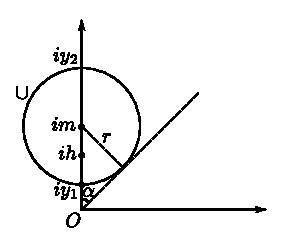
\includegraphics{vol29-fig/fig29-4.eps}
\smallskip
\caption{}
\label{chap1:fig4}
\end{figure}
$$
y_1 = h e^{-\rho}, \quad y_2 = h e^{\rho}
$$
implying that 
\begin{align*}
m & = \frac{1}{2} (y_1+y_2) = h \cosh \rho \tag{10}\label{eq1:10}\\
r & = \frac{1}{2} (y_2-y_1) = h \sinh \rho \tag{11}\label{eq1:11}
\end{align*}

Consequently, the circle $U$ is represented by
$$
|\tau -ih \cosh \rho| \ h \sinh \rho.
$$\pageoriginale

Further, we have 
\begin{equation*}
\sin \alpha = \frac{r}{m} = \tanh \rho, \tag{12}\label{eq1:12}
\end{equation*}
which is independent of $h$ showing that 
$$
|\frac{x}{y}| = \tan \alpha = \sinh \rho
$$
is the locus of those points at a distance $\rho$ from the line
$x=0$. In particular, if the centre of the circle $U$ is $i$, then its
equation is 
\begin{gather*}
|\tau-i \cosh \rho|= \sinh \rho, \quad \text{with} \quad \rho = \rho
(\tau, i)\\
\text{or } x^2 + (y-\cosh \rho)^2 = \sinh^2 \rho \Longrightarrow \cosh
\rho =\frac{x^2+y^2+1}{2y}
\end{gather*}

Moreover, $|z|^2 = \left|\dfrac{\tau - i}{\tau + i} \right|^2 =
\dfrac{x^2+y^2+ 1 - 2y}{x^2+y^2+1+2y} = \dfrac{\cosh \rho-1}{\cosh
  \rho + 1} = \tau h^2 \dfrac{\rho}{2}$. So the hyperbolic polar
coordinates can be introduced by 
\begin{equation*}
\frac{\tau - i }{\tau + i} = \tanh 
\frac{\rho}{2} \cdot e^{i0} \tag{13}\label{eq1:13}
\end{equation*}
We have already defined a metric on $\mathfrak{L}$, namely $\delta
(z_1, z_2)=\rho(\tau_l, \tau_2)$, where $z_i = A <\tau_i>$, $i = 1,
2$. In particular, we have 
$$
\delta = \delta (z,0) = \rho (\tau, i), \quad \delta^{\ast} = \delta
(z^{\ast},0) = \rho (\tau^{\ast}, i),
$$
where $z^{\ast} = \dfrac{\bar{\alpha} z+ \bar{\beta}}{\beta z +
  \alpha} = L <z>$. This gives an interesting geometric interpretation
for the expression $|\beta z + \alpha|$. We have seen that
$l - |z|^2 = 1 -\tanh^2 \delta/2 = \cosh^{-2} \delta/2$, from which it
can be shown easily that 
$$
l -|z^{\ast}|^2 = \frac{l-|z|^2}{|\beta z + \alpha|^2}. 
$$

Therefore \pageoriginale
$$
\frac{\cosh \delta^{\ast}/2}{\cosh \delta/2} = |\beta z + \alpha|.
$$

Because of the invariance of $\delta(z_l, z_2)$ by $\Omega_0$, $|\beta
z + \alpha|=1$ if and only if 
$$
\delta (z, L^{-1}<0>) = \delta (z^{\ast},0) = \delta (z,0)
$$
i.e. $z$ has the same hyperbolic distance from $0$ and $L^{-1}<0> =
-\bar{\beta}/\bar{\alpha}$.


\section{Discontinuous groups of motions}\label{chap1:sec2}%%% 2

Let $X$ be a topological space and $G$ a group acting on $X$ i.e., 
\begin{itemize}
\item[{\rm i)}] $gx$ for $g\in G$ and $x\in X$ belongs
  to $X$ and is uniquely defined, 

\item[{\rm ii)}] $g_l(g_2 x)=(g_lg_2)x$ for $g_l,g_2\in G$ and
  $x\in X$ and 

\item[{\rm iii)}] $ex=x$, where $e$ is the unit element of $G$.
\end{itemize}

\begin{defi*}
Two points $x_l, x_2$ of $X$ are said to be equivalent with respect to
$G$ if there exists an element $g$ in $G$ such that $g(x_l)=x_2$. It
is obvious that the set of points $\{gx |g \; \in G\}$ is a
\textit{complete set of equivalent points}.
\end{defi*}

\begin{defi*}
The group $G$ is said to \textit{act discontinuously on} $X$, if no
set of equivalent points has a limit point in $X$. Here, we consider
$g_lx$ and $g_2x$ with $g_l \neq g_2$ as different elements of the set
of points equivalent to $x$ even if $g_l x=g_2x$. 
\end{defi*}

In particular, if $G$ is a topological group, then $G$ can be
considered as acting on itself. We say that $G$ is \textit{discrete},
if $G$ acts discountinuously on itself.

\begin{lem}
A topological \pageoriginale group $G$ is discrete if and only if
there exists a 
neighbourhood of the unit element containing only a finite number of
elements. 
\end{lem}

\begin{proof}
For the sake of simplicity, we assume that $G$ satisfies the first
axiom of countability.
\begin{itemize}
\item[{\rm (i)}] Let every neighbourhood of the unit element $e$ in
  $G$ contain infinitely many elements. We can then choose a sequence
  $\{g_n\}$ in $G$ converging to $e$ with $g_n \neq g_{n+1}$ for all
  $n\geq 1$. Hence, for every $x$ in $G$, the sequence $\{g_n x\}$
  converges to $x$ as $n$ tends to infinity i.e. the set $\{gx
  |g \; \in G\}$ of elements in $G$ equivalent to $x$ has $x$ as a
  limit point, implying that $G$ is not discrete.

\item[{\rm (ii)}] Let $G$ be not discrete, so that $G$ contains a
  subset $\{gx |g \; \in G\}$ of elements equivalent to $x$ in $G$
  having a limit point, say $b$. Thus, we can find in $G$ a sequence
  $\{g_nx\}$ converging to $b$ as $n$ tends to infinity, with the
  property that $g_n \neq g_{n+1}$ for every $n\geq 1$. Then clearly
  $\{g_n x b^{-l}\}$ converges to the unit element $e$ and so does the
  sequence $\{bx^{-l}g^{-1}_{n+1}\}$. This leads us to a (non-trivial)
  infinite sequence $\{g_n g^{-1}_{n+1}\}$ converging to $e$. It
  follows that every neighbourhood of $e$ contains infinitely many
  elements. Our lemma is proved. 

In the sequel, we take $X$ to be the hyperbolic plane and $G$ to be
$\Omega$ or $\Omega_0$ according as $X = \mathfrak{H}$ or
$\mathfrak{L}$. The action of $G$ on $X$ in either case has been
defined already in $\S 1$.
\end{itemize}
\end{proof}

\begin{thm}
A subgroup $\Gamma$ of $G$ acts discontinuously on $X$ if and only if
$\Gamma$ is discrete.
\end{thm}

\begin{proof}
We work \pageoriginale with $X=\mathfrak{L}$ for the proof.
\begin{itemize}
\item[{\rm (i)}] Let $\Gamma$ act discontinuously on
  $\mathfrak{L}$. Then we shall show that $\Gamma$ is discrete. Let,
  if possible, $\Gamma$ be not discrete. Then there exists a 
sequence $ \left\{ S_n = \begin{bmatrix}
\bar{\alpha}_n & \bar{\beta}_n\\
\beta_n & \alpha_n\end{bmatrix}\right\}$ in $\Gamma$ such
  that $S_n \neq S_{n+1} $ and $S_n \to E = \begin{pmatrix}1&0\\
0&1\end{pmatrix}$ as $n\to\infty$. This implies that
$$
\alpha_n \to 1 \; \text{ and } \;  \beta_n \to 0 \text{ i.e. }
S_n<0>=\bar{\beta}_n/ \alpha_n \to 0\;  \text{ as }\;  n \to \infty.
$$

Thus the set of equivalent points $\{S<0>|S\in \Gamma\}$ has a
limit point, contradicting the discontinuous action of $\Gamma$. Hence
$\Gamma$ is necessarily discrete.

\item[{\rm (ii)}] Let now $\Gamma$ be discrete. If $\Gamma$ does not
  act discontinuously on $\mathfrak{L}$, then there exists a point $z$
  in $\mathfrak{L}$ such that the set $\{S<z>|S\in \Gamma\}$
  has a limit point say $z^{\ast}$. Therefore we can find a sequence
$\left\{ S_n = \begin{bmatrix}
\bar{\alpha}_n & \bar{\beta}_n\\
\beta_n & \alpha_n  \end{bmatrix}  \right\}$ in $\Gamma$ with $S_n
  \neq S_{n+1}$ such that $S_n <z> \to z^{\ast}$ as $n =  \infty$. Let
  $z_n = S_n <z> = \dfrac{\bar{\alpha}_nz+\bar{\beta}_n}{\beta_n z +
    \alpha_z}$. Then 
\begin{gather*}
1-|z_n|^2 = \frac{1-|z|^2}{|\beta_nz+\alpha_n|^2} \to 1
-|z^{\ast}|^2\\
\Longrightarrow |\beta_n z + \alpha_n| \to
\sqrt{\frac{1-|z|^2}{l-|z^{\ast}|^2}} \text{ as } n \to \infty.
\end{gather*}

Since $\left|\dfrac{\beta_n}{\alpha_n}\right| < 1, |\beta_n z +
\alpha_n| = |\alpha_n| \left|\frac{\beta_n}{\alpha_n} z+1\right| \geq
|\alpha_n| (1-|z|)$. This shows that $|\alpha_n|$ and therefore
$|\beta_n|$ is bounded. Therefore we can find a subsequence
$\{S_{k_n}\}$ of $\{S_n\}$ such that $\{S_{k_n} S^{-1}_{k_{n+1}}\} \to
E$ as $n\to \infty$. But this is contrary to the discreteness of
$\Gamma$; therefore, $\Gamma$ acts discontinuously on $\mathfrak{L}$.
\end{itemize}
\end{proof}

\begin{defi*}
A conformal \pageoriginale transformation of the hyperbolic plane with
the corresponding matrix $S\neq \pm E$ is said to be
\textit{hyperbolic} or \textit{elliptic} or \textit{parabolic}
according as the two fixed points of the transformation are distinct
and lie on the boundary of the hyperbolic plane or the two fixed
points are inverse points with respect to the boundary circle of the
hyperbolic plane or the two fixed points coincide.
\end{defi*}

It can be proved easily that if the determinant $|S|$ of $S$ equals
$1$, then 
\begin{equation*}
\rho^2 (S) = (\sigma(S))^2 
\begin{cases}
> 4 & \text{ if $S$ is hyperbolic},\\
< 4 & \text{ if $S$ is elliptic},\\
= 4 & \text{ if $S$ is parabolic},
\end{cases} \tag{1}\label{eq2:1}
\end{equation*}
where $\sigma(S)$ denotes the trace of $S$.

By a \textit{hyperbolic group} of transformations of the hyperbolic
plane we mean a group consisting wholly of hyperbolic transformations
except for $E$ and possibly $-E$ as well. We have the following
remarkable theorem for this hype of groups.

\begin{thm}
If a subgroup $\Gamma$ of $\Omega$ is a non-commutative hyperbolic
group, then $\Gamma$ acts discontinuously on the hyperbolic plane $X$.
\end{thm}

\begin{proof}
We shall take the upper half-plane $\mathfrak{H}$ as a model for
$X$. Now $\Gamma$ contains a hyperbolic element $S\neq \pm E$ with
fixed points $\omega, \omega' \neq \omega$. For $V$ in $\Omega$
defined by $V<\tau>=(\tau - \omega) (\tau-\omega')^{-l}$, let
$S^{\ast}=VSV^{-1}$ and $\Gamma^{\ast}=V\Gamma V^{-l}$. Then
$\sigma(S^{\ast}) =\sigma(S)$ so that $S^{\ast}$ is again hyperbolic
and further $\Gamma^{\ast}$ is also a hyperbolic group, which is
discrete if and only if $\Gamma$ is discrete. Thus passing over to
$\Gamma^{\ast}$ if necessary, we may assume that \pageoriginale $S$
has already 0 and $\infty$ as its fixed points, so that
$S=\begin{pmatrix}
\ell & 0 \\
0 & \ell^{-1}
\end{pmatrix}$ with $\ell \neq \pm 1$.

If possible, let $\Gamma$ no act discontinuously on
$\mathfrak{H}$. then by theorem 1, $\Gamma$ is not discrete and
therefore contains a sequence $\{T_n\}$ of elements $T_n \neq \pm E$
converging to $E$. We will show under the given circumstances, that
all but finitely many $T_n$ are diagonal. For $T_m = \begin{pmatrix}
a&b\\
c&d
\end{pmatrix}$, consider the commutators $C_m = ST_m S^{-1} T^{-1}_m$
and $D_m = SC_m S^{-1}C^{-1}_m$. If is easily checked that 
\begin{align*}
C_m & = \begin{pmatrix}
ad-bc \ell^2 & ab (\ell^2-1)\\
cd (\ell^{-2}-1) & ad-bd\ell^{-2}
\end{pmatrix}\\
& = \begin{pmatrix}
1+bc(1-\ell^2) & ab(\ell^2-1)\\
cd (\ell^{-2}-1) & 1+bc (1-\ell^{-2})
\end{pmatrix}
\end{align*}

Since $\Gamma$ is hyperbolic, the element $C_m$ is hyperbolic if $C_m
\neq \pm E$. In any case, 
$$ 
\sigma^2(C_m) = (2+2bc - bc (\ell^2 + \ell^{-2}))^2 = (2-bc
(\ell-\ell^{-1})^2)^2 \geq 4.
$$

Similarly, we have  
$$
\sigma^2(D_m) = (2-ab(\ell^2-1) cd (\ell^{-2}-1) (\ell-\ell^{-1})^2)^2
= (2+abcd (\ell-\ell^{-1})^4)^2 \geq 4.
$$

Since $\{T_n\}$ converges to $E,\{C_n\}$ converges to $E$ so that
$1+bc(1-\ell^2)$ tends to $1$. Since $\ell \neq \pm 1$ is fixed, this
means that $bc$ tends to 0. We claim that $bc=0$ for all large enough
$m$. In fact, if $bc$ is positive and sufficiently small, we have a
contradiction from $\sigma^2(C_m)=(2-bc(\ell-\ell^{-1})^2)^2<4$. Since
$ad-bc=1$, $ad$ tends to $1$ and hence \pageoriginale disregarding
finitely many $m$, we can suppose that $ad > 0$, so that $abcd$ has
the same sign as $bc$. Let now $bc<0$, if possible. Then considering
$D_m$ instead of $C_m$, we see that $abcd$ tends to 0 as $m$ tends to
$\infty$. But from $bc <0$, we obtain that $abcd<0$ and $|abcd|$ is
small for all large $m$, so that $\sigma^2(D_m)<4$, a contradiction
again. Thus, for all large $m$, $bc =0$ and therefore $ad=1$. Now
$\sigma(C_m)=2ad =2$ and since $\Gamma$ is hyperbolic, this means that
$C_m = E$, for all large $m$ i.e. $ab=cd =0$. Since $ad=1$, we have
$b=c=0$ i.e. $T_m$ is diagonal, for all large $m$, as required to be
proved.

Dropping finitely many $T_m$, we have in $\Gamma$, a sequence
$\{T_n\}$ of diagonal matrices $T_n = \left(\begin{smallmatrix}
\ell_n & 0 \\ 0 & 1/\ell_n\end{smallmatrix}\right)$ with $\ell_n \neq
\pm 1$. Let now $F= \left(\begin{smallmatrix}
p & q\\r & s\end{smallmatrix}\right)$ be an arbitrary element of
$\Gamma$. To the sequence $\{T_n F T^{-1}_n F^{-1}\}$ (of commutators)
converging to $E$ (as $n\to \infty$), we apply the same arguments as
to $\{C_m\}$ above. Then we can conclude that necessarily $q=r=0$ and
$F$ is diagonal. In other words, $\Gamma$ consists entirely of
diagonal matrices and is hence commutative, a contradiction. Thus
$\Gamma$ necessarily acts discontinuously on $X$.
\end{proof}

\section{Fundamental domain}\label{chap1:sec3}
Let $\Gamma$ be a discrete group of motions of the hyperbolic plane.

\begin{defi*}
A point-set $\mathfrak{F}$ of the hyperbolic plane is called a
{\em fundamental domain} for $\Gamma$ if
\begin{enumerate}
\renewcommand{\labelenumi}{\theenumi)}
\item $\mathfrak{F}$ contains at least one point from each set of
  equivalent points with respect to $\Gamma$ and 

\item If $z\in \mathfrak{F} \cap \mathfrak{F}_S$
  ($\mathfrak{F}_S =$ Image of $\mathfrak{F}$ by $S$), then $z$ is a
  boundary point of $\mathfrak{F}$ and $\mathfrak{F}_S$ provided $S
  \neq \pm E$. 
\end{enumerate}
\end{defi*}

In the \pageoriginale following, we shall give a construction of a
fundamental domain for $\Gamma$ by geometrical methods. First of all,
we observe that $\Gamma$ is countable. For, the number of matrices $S
= \left(\begin{smallmatrix}
\bar{\alpha} & \bar{\beta}\\
\beta & \alpha \end{smallmatrix} \right)$ with $\alpha \bar{\alpha} \leq
n $ ($n$ a natural number) is finte, because if the number of such
matrices were infinite, then $\alpha\bar{\alpha}\leq n$ and $\beta
\bar{\beta}=\alpha\bar{\alpha}-l<n$ will imply that $\Gamma$ is not
discrete. Since every element $S\in \Gamma$ different from
$\pm E$ can have atmost one fixed point in $\mathfrak{L}$ and $\Gamma$
is countable, there exists a point $\zeta \in \mathfrak{L}$
which is not a fixed point of any element $S$ of $\Gamma$ different
from $\pm E$. In the following, we set $S<\zeta> = \zeta_S$. We shall
show that the set $\mathfrak{F}$ defined by
\begin{equation*}
\mathfrak{F} = \{z|\delta(z,\zeta) \leq \delta (z,\zeta_S) \text{ for
} S \in \Gamma, z\in \mathfrak{L}\} \tag{1}\label{eq3:1}
\end{equation*}
is a fundamental domain for $\Gamma$. It is obvious that
$\mathfrak{F}$ consists of all points $z$, whose distance from $\zeta$
is not greater than the distance from the equivalent points
$\zeta_S$. Obviously, we have 
\begin{align*}
\mathfrak{F}_T & = \{T<z>|\delta (z,\zeta) \text{ for } S \in \Gamma,
z\in \mathfrak{L}\}\\
& = \{z|\delta (T^{-l}<z>,\zeta) \leq \delta(T^{-l} <z>, \zeta_S)
\text{ for }
S \in \Gamma, z \in \mathfrak{L}\}\\
& = \{z|\delta(z,\zeta_T) \leq \delta (z,\zeta_{TS}) \text{ for } S \in
\Gamma, z \in \mathfrak{L}\}\\
& = \{z|\delta (z,\zeta_T) \leq \delta (z,\zeta_S) \text{ for } S \in
\Gamma, z \in \mathfrak{L}\}.
\end{align*}

We now claim that 
$$
\mathfrak{L} = \bigcup\limits_{\pm T \in \Gamma} \mathfrak{F}_T.
$$

Indeed, for an arbitrary $z\in \mathfrak{L}$ the set $\{\delta
(z,\zeta_S)|S\in \Gamma\}$ has a minimum because of the
discreteness of $\Gamma$, i.e. $\delta(z,\zeta_T)\leq \delta
(z,\zeta_S)$ for some $T$ in $\Gamma$ and for all $S$ in $\Gamma$;
therefore, $z\in \mathfrak{F}_T$. In particular,
$\mathfrak{F}$ contains atleast \pageoriginale one point from each set
of equivalent points. In order to prove the second condition for
$\mathfrak{F}$ to be a fundamental domain, we proceed as follows. Let
$g_S$ for $S\neq \pm E$ denote the locus of points $z \in
\mathfrak{L}$ such that 
$$
\delta(z,\zeta) = \delta(z,\zeta_S).
$$

This is the equation of an orthogonal circle, which for $\zeta = 0$ as
shown in $\S 1$ can be represented by $|-\beta z + \bar{\alpha}|=1$ if
$S = \left(\begin{smallmatrix}  \bar{\alpha} & \bar{\beta}\\
\beta & \alpha
\end{smallmatrix}\right)$. The line $g_S$ decomposes the hyperbolic
plane into two parts. We denote by $\mathfrak{L}_S$ the closed half
plane which contains $\zeta$. In fact, 
$$
\mathfrak{L}_S = \{z\in \mathfrak{L} |\delta(z,\zeta) \leq \delta
(z,\zeta_S)\}. 
$$

Therefore $\mathfrak{F} = \bigcap\limits_{\pm S \in \Gamma}
\mathfrak{L}_S$. In particular, since each $\mathfrak{L}_S$ is a
convex set and an arbitrary intersection of convex sets is convex,
$\mathfrak{F}$ is a convex set. Moreover, it can be verified easily
that the boundary of $\mathfrak{F}$ in $\mathfrak{L}$ consists of some
segments of the hyperbolic straight lines $g_T$ for $T \in
\Gamma$. In other words, $z$ is a boundary point of $\mathfrak{F}$ if
and only if $\delta(z,\zeta) \leq \delta (z, \zeta_S)$ for $S
\in \Gamma$ and equality holds atleast for one $S \neq \pm
E$. Thus if $z\in \mathfrak{F} \cap \mathfrak{F}_T$, then
necessarily, we have $\delta (z,\zeta)\leq \delta (z,\zeta_S)$ and
$\delta (z,\zeta_T) \leq \delta (z,\zeta_S)$ for $S\in
\Gamma$. Taking $S=T$ in the first inequality and $S=E$ in the second,
we obtain that 
$$
z \in \mathfrak{F} \cap \mathfrak{F}_T \Longrightarrow \delta
(z,\zeta) = \delta (z,\zeta_T)
$$
showing that $z$ is a boundary point of $\mathfrak{F}$ and
$\mathfrak{F}_T$. Hence the set defined in \eqref{eq3:1} is a fundamental
domain for $\Gamma$. Moreover, we shall now prove that only finitely
many lines $g_T$ for $T$ in $\Gamma$, constituting the boundary of
$\mathfrak{F}$, intersect a given compact set $K$. Let $K$ be
contained in the circle $U = \{z|\delta (z,\zeta) \leq R, z\in
\mathfrak{L}\}$. \pageoriginale If $z \in g_T \cap U$, then we
must have 
\begin{gather*}
R \geq (z,\zeta) \geq \frac{1}{2} \delta (\zeta, \zeta_T)\\
\text{or} \delta (\zeta, \zeta_T) \leq 2 R.
\end{gather*}

But $\Gamma$ is discontinuous and therefore only finitely many $T$
exist for which $\delta(\zeta, \zeta_T)\leq 2R$. We thus conclude
that $\mathfrak{F}$ as defined in \eqref{eq3:1} is a convex set bounded by a
countable number of hyperbolic lines, only a finite number of which
intersect a given compact set. We call such a fundamental domain
$\mathfrak{F}$ a \textit{normal fundamental domain} with the centre
$\zeta$. The area of $\mathfrak{F}$ is given by 
$$
\mathfrak{I} (\mathfrak{F}) =\lim\limits_{\rho\to \infty}
4\int\limits_{\substack{\delta(z,\zeta)\leq \rho\\z\in
    \mathfrak{F}}} \frac{du dv}{(l-u^2 -v^2)^2}.
$$

This integral may be an improper integral and can have an infinite
value. If the value is infinite, then the fundamental domain has limit
points on the boundary of the hyperbolic plane. If the fundamental
domain is compact, its area is finite; the converse is not true in
general. However, we have the following 

\begin{thm}\label{chap1:thm3}
If $\Gamma$ is a discrete group of motions of the hyperbolic plane
containing no parabolic motions and having a normal fundamental domain
$\mathfrak{F}$ with finite area, then $\mathfrak{F}$ is compact.
\end{thm}

\begin{proof}
Throughout the proof, the hyperbolic plane will be represented by
$\mathfrak{L}$. We decompose the boundary of $\mathfrak{F}$ in
$\mathfrak{L}$ into connected components, the number of which will be
atmost countable. The proof is given in six steps.
\begin{enumerate}
\renewcommand{\labelenumi}{\theenumi)}
\item If there\pageoriginale exists one connected component which is a
  closed curve, then this cannot have double points, in view of
  $\mathfrak{F}$ being convex. So this connected component represents
  a polygon. Since $\mathfrak{F}$ is convex and therefore simply
  connected, $\mathfrak{F}$ is in the interior of this polygon and is
  obviously compact. We exclude this case from our
  considerations. Starting from a boundary point of $\mathfrak{F}$ in
  $\mathfrak{L}$ (which exists by the construction of $\mathfrak{F}$),
  if we move along the boundary of $\mathfrak{F}$ in one of the two
  possible directions, then the following two possibilities can occur:
\begin{itemize}
\item[{\rm (a)}] we come across only a finite number of vertices
  i.e. there exists a last edge reaching the boundary of
  $\mathfrak{L}$,

\item[{\rm (b)}] we meet an infinite number of vertices.
\end{itemize}

The case in which we come back to the starting point has already been
discussed above. Let 
$$
\ldots \ldots, z_{-1}, z_0, z_1, z_2, \ldots \ldots
$$
denote the vertices of one of the connected components of
$\mathfrak{F}$. Here, if the sequence terminates on the right with
$z_r$, then through $z_r$ pass two edges of $\mathfrak{F}$, one
joining the point $z_{r-1}$ to $z_r$ and the other reaching the
boundary of $\mathfrak{L}$. If $z_{r+1}$ is the point of intersection
of the boundary of $\mathfrak{L}$ with the edge through $z_r$ reaching
the boundary of $\mathfrak{L}$, we define $z_{r+1}$ to be a vertex of
the fundamental domain $\mathfrak{F}$. Similarly, if the sequence
terminates on the left with $z_{-r}$, we define the point $z_{-r-1}$
to be a vertex of $\mathfrak{F}$. The triangle $\Delta_k$ with the
vertices $\zeta$ (the centre of $\mathfrak{F}$), $z_k$ and $z_{k+1}$
is contained in $\mathfrak{F}$, since $\mathfrak{F}$ is a convex set.

Let \pageoriginale $\alpha_k, \beta_k$ and $\gamma$ 
(as in figure~\ref{chap1:fig5} be the angles of $\Delta_k$. Then

\begin{figure}[H]
\centering
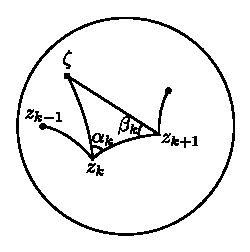
\includegraphics{vol29-fig/fig29-5.eps}
\smallskip
\caption{}
\label{chap1:fig5}
\end{figure}

$$
\mathfrak{I} (\Delta_k) = \pi - \alpha_k - \beta_k -\gamma_k.
$$

If $z_k$ respectively $z_{k+1}$ belongs to the boundary of
$\mathfrak{L}$, then $\alpha_k$ respectively $\beta_k$ is equal 
to 0. Let $\omega_k =\alpha_k + \beta_{k-1}$.

Then, because of the convexity of $\mathfrak{F}$, we have 
\begin{equation*}
0 < \omega_k < \pi. \tag{2}\label{eq3:2}
\end{equation*}

Summing the areas of the triangles $\Delta_k$ for $p \leq k \leq q$,
we obtain 
\begin{gather*}
\mathfrak{I}_{p,q} = \sum^q_{k=p} \mathfrak{I} (\Delta_k) =
\sum^q_{k=p} (\pi - \alpha_k - \beta_k - \gamma_k)\\
\text{or } \mathfrak{I}_{p,q} + \sum^q_{k=p} \gamma_k = \pi - \alpha_p
- \beta_q + \sum^q_{k=p+1} (\pi - \omega_k). \tag{3}\label{eq3:3}
\end{gather*}

But
\begin{equation*}
\mathfrak{I}_{p,q} \leq \mathfrak{I} (\mathfrak{F}) < \infty, \quad
A_{p,q} := \sum^q_{k=p} \gamma_k \leq 2\pi, \tag{4}\label{eq3:4}
\end{equation*}
and therefore, in case (b), the sequences $\mathfrak{I}_{p,q}$ and
$A_{p,q}$ converge when $p \to -\infty$ and $q\to \infty$. Since
$\alpha_p, \beta_q <\pi$ from \eqref{eq3:2}, the series
$\sum\limits^q_{k=p+1}(\pi-\omega_k)$ converges when $p\to -\infty$ and $q\to
\infty$. The convergence of the sequence $\mathfrak{I}_{p,q}$ implies
the convergence of $\alpha_p$ when $p\to -\infty$ and $\beta_p$ when
$q \to \infty$. Let us write
\begin{equation*}
\lim_{p\to -\infty} \alpha_p = \alpha_{-\infty}, \quad
\lim_{q\to\infty} \beta_q = \beta_{\infty}. \tag{5}\label{eq3:5}
\end{equation*}

In the case of the possibility (a), we choose $p$ to be minimal and $q$
to \pageoriginale be maximal and then $\alpha_p = \beta_q =0$. We
shall now show that the limiting values of $\alpha_p$ and $\beta_q$ in
\eqref{eq3:5} satisfy the inequalities 
\begin{equation*}
\alpha_{-\infty} \leq \frac{\pi}{2}, \quad \beta_{\infty} \leq
\frac{\pi}{2}. \tag{6}\label{eq3:6}
\end{equation*}

Let $r_k = \delta (z_k, \zeta)$. Then if there exists no extremal $p$
(respectively $q$), we have 
$$
r_k \to \infty, \text{ for } k \to -\infty (\text{respectively } k \to
\infty).
$$

For, only a finite number of edges $\widehat{z_kz_{k+1}}$
($\widehat{z_kz_{k+1}}$) denoting the hyperbolic line joining $z_k$ and
$z_{k+1}$) can meet a given compact set. We must have 
\begin{equation*}
r_k < r_{k+1} \text{ for infinitely many $k$}, \tag{7}\label{eq3:7}
\end{equation*}
since, otherwise, the sequence $r_k$ will be bounded. We now prove
that, in the triangle $\Delta_k$ for which $r_k < r_{r+1}$, opposite
to the greater side we have the greater angle (as in Figure~\ref{chap1:fig6} i.e.
\begin{equation*}
\beta_k < \alpha_k. \tag{8}\label{eq3:8}
\end{equation*}
%%%

\begin{figure}[H]
\centering
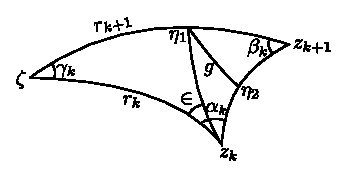
\includegraphics{vol29-fig/fig29-6.eps}
\smallskip
\caption{}
\label{chap1:fig6}
\end{figure}

Let $g$ denote the perpendicular bisector of $\widehat{z_k z_{k+1}}$
(in the sense of hyperbolic geometry). Since $z_k < z_{k+1}$, it
follows that $\eta_1$, the point of intersection of $g$ and the line
through $\zeta$ and $z_{k+1}$ lies between $\zeta$ and \pageoriginale
$z_{k+1}$. This means that the angle $\in$ (see Figure~\ref{chap1:fig6} is
positive. It is obvious that the triangles $<z_k \eta_1 \eta_2>$ and
$<\eta_l \eta_2 z_{k+1}>$ are congruent in the hyperbolic
sense. Therefore we have $\beta_k = \alpha_k-\in$, which
proves our assertion \eqref{eq3:8}. But $\mathfrak{I}(\Delta_k) + \gamma_k = \pi
- \alpha_k -\beta_k >0$; therefore, from \eqref{eq3:8}, we conclude that 
\begin{equation*}
\beta_k <\frac{\pi}{2} \text{ for infinitely many } k. \tag{9}\label{eq3:9}
\end{equation*}

Our assertion $\beta_{\infty} \leq \dfrac{\pi}{2}$ in \eqref{eq3:6} now follows
trivially. Similarly, it can be proved that $\alpha_{-\infty} \leq
\dfrac{\pi}{2}$. 

\item Let $m$ denote the maximal $q$ if it exists, and otherwise, set
  $m=\infty$; let $n$ denote the minimal $p$ if in exists and
  otherwise set $n=-\infty$. From \eqref{eq3:3}, it follows that 
\begin{equation*}
\sum^m_{k=n} \gamma_k + \sum^m_{k=n} \mathfrak{I} (\Delta_k) = \pi -
\alpha_n -\beta_{m} + \sum^m_{k=n+1} (\pi-\omega_k). \tag{10}\label{eq3:10}
\end{equation*}

If we sum both sides of \eqref{eq3:10} over all the connected components of the
boundary of $\mathfrak{F}$, then we still have
\begin{equation*}
\sum_k \gamma_k \leq 2\pi \text{ and } \sum_k \mathfrak{I} (\Delta_k)
\leq \mathfrak{I} (\mathfrak{F}) < \infty. \tag{11}\label{eq3:11}
\end{equation*}

But $\pi - \alpha_n - \beta_m \geq 0$, therefore the series $\sum_k
(\pi-\omega_k)$ of positive terms is convergent and for a given
$\in >0$, we have
\begin{equation*}
0 < (\pi-\omega_k) < \in \text{ for almost all } k. \tag{12}\label{eq3:12}
\end{equation*}

\item We have defined the set $\mathfrak{F}$ by means of the
  inequalities 
$$
\delta(z, \zeta) \leq \delta (z,\zeta_S) \text{ for } S \in
\Gamma. 
$$

If equality holds precisely for one $S \neq \pm E$ i.e. if $z$ lies
exactly on one perpendicular bisector, then $z$ is a boundary point of
$\mathfrak{F}$ and not a vertex. \pageoriginale Since the edge
$\widehat{z_k z_{k+1}}$ of $\mathfrak{F}$ is a perpendicular bisector
of $\widehat{\zeta \zeta_{A}}$ for some $A \in \Gamma$, we
have, for any point $z$ on this edge different from $z_k$ and $z_{k+1}$,
\begin{align*}
 \delta (z,\zeta) & = \delta (z,\zeta_A) \text{ and } \delta(z,\zeta) <
\delta (z,\zeta_S) \text{ for } S \neq \pm A, \pm E,\\
\text{or } \quad 
 \delta (z,\zeta_A) & = \delta
(z,\zeta_{A^{-1}A} ) \text{ and } \delta (z,\zeta_A) \leq \delta
(z,\zeta_{SA}) \text{ for } S \neq \pm A^{-1}, \pm E. 
\end{align*}

This shows that $z$ is a boundary point of $\mathfrak{F}_A$ and not a
vertex. Moreover $z_k$ and $z_{k+1}$ are necessarily vertices of
$\mathfrak{F}_A$. We now assert that a vertex of $\mathfrak{F}$, say
$z_0$, can be a vertex of only finitely many images of $\mathfrak{F}$
by elements of $\Gamma$. Let, if possible, $z_0$ be a vertex of
$\mathfrak{F}_{A_i}(i=1,2,\ldots)$ with $A_i \in \Gamma$. Then
we have 

\begin{figure}[H]
\centering
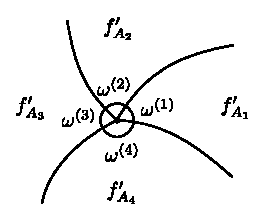
\includegraphics{vol29-fig/fig29-7.eps}
\smallskip
\caption{}
\label{chap1:fig7}
\end{figure}
$$
\begin{matrix} 
\delta (z_0, \zeta) & = \delta(z_0, \zeta_{A_1})\\ 
\delta (z_0, \zeta_{A_l}) & = \delta(z_0, \zeta_{A_2})\\
\hdotsfor{2}\\
\delta(z_0, \zeta_{A_i}) & =\delta(z_0, \zeta_{A_{i+1}})
\end{matrix}
$$
and so on. Thus we obtain that 
$\delta(z_0, \zeta) = \delta (z_0,\zeta_{A_i})$ for $i=1,2,\ldots$
i.e. the points $\zeta_{A_i}$ lie on the hyperbolic circle with the
radius $\delta(z_0, \zeta)$. This implies, because of the discreteness
of $\Gamma$, that there can exist only finitely many such $A_i$,
proving our assertion above. Let $\mathfrak{F}_{A_i}, i = 1, 2, \ldots,
r (r\geq 3)$ be all the images of $\mathfrak{F}$ with $z_0$ as a
vertex and let $\omega^{(i)}$ denote the angle of $\mathfrak{F}_{A_i}$
at $z_0$. Then 
\begin{equation*}
\omega^{(1)} + \omega^{(2)} + \cdots + \omega^{(r)} = 2\pi \tag{13}\label{eq3:13}
\end{equation*}

Since $A^{-l}_i <z_0>$ will be some vertex of $\mathfrak{F}$, say $z_j
\omega^{(i)}$ must coincide with $\omega_j$. 

We assume in the rest of the proof that $-E \in \Gamma$,
without loss of generality and denote $\Gamma/\{\pm E\}$ by
$\bar{\Gamma}$. 

\item Let \pageoriginale $B_i <z_0> (i=1,2,\ldots, S)$ with $B_i
  \in \Gamma$ be the complete set of different vertices of
  $\mathfrak{F}$ which are equivalent with $z_0$. Denote by $\Gamma_0$
  the subgroup consisting of those transformations of $\Gamma$ which
  leave $z_0$ fixed. Since $A^{-l}_i <z_0>$ with $A_i$ as defined
  above is a vertex of $\mathfrak{F}$, we have $A^{-l}_i <z_0> = B_j
  <z_0>$ i.e. $A_i B_j <z_0>=z_0$ for some $j$ with $1\leq j \leq s$
  and therefore $A_i B_j = L$ for some $L\in \Gamma_0$. The
  number of distinct transformations $A^{-1}_i = \pm B_j L^{-1}$ is
  $\ell s$, where $\ell$ is the order of $\bar{\Gamma}_0:=\Gamma_0/
  \{\pm E\}$; for, if $\pm B_j L^{-1}_1 = B_h L^{-1}_2$ for $L_k
  \in \Gamma_0(k=1,2)$, then $B_j <z_0>=B_h <z_0>$ and this is
  possible only if $j=h$, implying in turn that $\pm L_1 = L_2$. This
  shows that $r=\ell s$ and $\ell$ is finite; therefore
  $\bar{\Gamma}_0$ is a cyclic group. Let $\bar{\Gamma}_0$ be
  generated by the rotation $L_0$ of angle $2\pi/\ell$. Then
$$
\{\pm A^{-1}_i | i = 1, 2, \ldots, r\} = \{\pm B_j L^{-t}_0| j = 1, 2
, \ldots, s; t = 0,1, \ldots, \ell-l\}. 
$$

Since the fundamental domain $\mathfrak{F}$ has the angle
$\omega^{(j)}$ at the vertex $B_j <z_0>=B_j L^{-t}_0 <z_0>$, the image
$\mathfrak{F}_{A_i} = \mathfrak{F}_{L^t_0 B^{-1}_j}$ has the same
angle $\omega^{(j)}$ at $z_0$. Therefore, from \eqref{eq3:13}, it follows that 
\begin{equation*}
\omega^{(1)} + \omega^{(2)} + \cdots + \omega^{(s)} =
\frac{2\pi}{\ell} (s\ell \geq 3) \tag{14}\label{eq3:14}
\end{equation*}

But, by \eqref{eq3:12}, $\omega_k > \dfrac{2\pi}{3}$ for almost all $k$;
therefore, equation \eqref{eq3:13} can be satisfied only by a finite number of
systems $\omega_k$. Thus there exist only finitely many classes of
equivalent vertices of $\mathfrak{F}$, since each such class
corresponds uniquely to a subsystem of $\{\omega_k\}$ satisfying \eqref{eq3:14}
with some $\ell$ and further any two such subsystems are disjoint. We
conclude that every connected component of the boundary of
$\mathfrak{F}$ has finitely many vertices. From \eqref{eq3:10} with $\alpha_n =
\beta_m =0$ now, we obtain that the right hand side of \eqref{eq3:10} is at
least $\pi$. But the left hand side of \eqref{eq3:10} when summed over all
connected component\pageoriginale is finite. Therefore it follows
that the number of connected components of $\mathfrak{F}$ is finite.

\item We shall now show that no arc of the boundary of $\mathfrak{L}$
  can be contained in the boundary of $\mathfrak{F}$. Without loss of
  generality, we can assume that $\zeta=0$. Let us suppose that the
  arc $\widehat{AB}$ with the angle $\gamma>0$ belongs to the boundary
  of $\mathfrak{F}$. Then due to the convexity of $\mathfrak{F}$, the
  whole sector belongs to $\mathfrak{F}$. But this is impossible,
  since the area of this sector is infinite while $\mathfrak{F}$ has
  finite area. For the same reason, $\mathfrak{F}$ can at most have
  only finitely many improper vertices i.e. vertices on the boundary
  of $\mathfrak{L}$.

\begin{figure}[H]
\centering
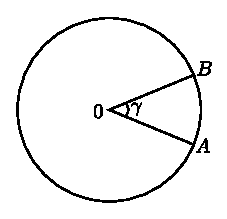
\includegraphics{vol29-fig/fig29-8.eps}
\smallskip
\caption{}
\label{chap1:fig8}
\end{figure}

\item We prove next that $\mathfrak{F}$ does not have any improper
  vertex. Here, for the first time, we shall make use of the
  assumption on $\Gamma$ that it does not contain parabolic
  transformations. Let $z_0$ be an improper vertex of $\mathfrak{F}$
  so that $|z_0|=1$. Since $\mathfrak{F}$ does not contain any arc of
  the boundary of $\mathfrak{L}$. two edges of $\mathfrak{F}$, say
  $g_0$ and $f_0$, touch each other at $z_0$. Let $\mathfrak{F}_{A_1}$
  be an image of $\mathfrak{F}$ by $A_1 \in \Gamma$, which has
  the edge $g_0$ in common with $\mathfrak{F}$. By the same argument
  as above, $\mathfrak{F}_{A_1}$ must have two edges $g_0$ and $g_1$
  touching at $z_0$. Proceeding in this way, we obtain $\ldots \ldots,
  \mathfrak{F}_{A_{-2}}, \mathfrak{F}_{A_{-1}}, \mathfrak{F}_{A_0},
  \mathfrak{F}_{A_1}, \mathfrak{F}_{A_2}, \ldots \ldots $ with $A_0=E$
  and $A_i \in \Gamma$ having $z_0$ as the common improper
  vertex. Obviously $A^{-1}_r<z_0>$ is an improper vertex of
  $\mathfrak{F}$. But $\mathfrak{F}$ has only finitely \pageoriginale
  many vertieces; therefore, there exist two integers $p$ and $q$
  with $p \neq q$ such that 
{\fontsize{10}{12}\selectfont
$$
A^{-1}_p <z_0> = A^{-1}_q <z_0> \Longrightarrow C<z_0> = z_0 \text{
  with } C = A_p A^{-1}_q \neq \pm E.
$$}\relax

Since, by assumption, $\Gamma$ does not contain any parabolic
transformation, the transformation $C$ which has a fixed point $z_0$
on $|z|=1$, ought to be hyperbolic. Let $z_1$ be the other fixed point
of $C$. Let, further, $\tau=T<z>$ be a transformation which maps the
unit disc onto the upper-half plane and the points $z_0,z_1$ to
$\infty, 0$ respectively. Then $C=T^{-1} \begin{bmatrix}
\lambda & 0 \\
0 & \lambda^{-1}\end{bmatrix}T$, with $\lambda \neq 0, \pm
1$. Clearly, the cyclic group generated by $TCT^{-1}$ maps the set
$\mathfrak{g} = \{\tau = x + iy,|x| \leq y ; \tau \in
\mathfrak{H}\}$ onto itself. Let $\mathfrak{F}_0$ be the fundamental
domain in $T^{-1}<\mathfrak{g}>$ of the cyclic group generated by $C$,
say, with $\lambda^2>1$, such that (see Figure~\ref{chap1:fig9}
$$
T <\mathfrak{F}_0> = \{\tau | \tau = x+ iy, 1 \leq |\tau| \leq
\lambda^2, |x| \leq y\}.
$$

\begin{figure}[H]
\centering
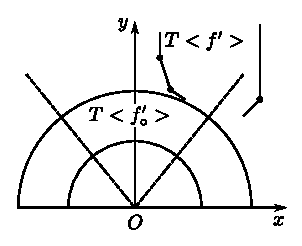
\includegraphics{vol29-fig/fig29-9.eps}
\smallskip
\caption{}
\label{chap1:fig9}
\end{figure}

Then $\mathfrak{F}_0$ is a compact set in the hyperbolic plane and
therefore there exists a constant $M$ such that $\delta(z^{\ast},
\zeta) \leq M$ for $z^{\ast} \in \mathfrak{F}_0$.

Since $T<\mathfrak{F}>$ has $\infty$ as a boundary point, there exists
a point $z\in \mathfrak{F}$ such that $\delta (z,\zeta)>M$ and
$T<z>\in y$. This implies that $C^p<z>$  belongs to
$\mathfrak{F}_0$ for some integer $p$  and therefore 
$$
\delta (C^p <z>, \zeta) = \delta (z,\zeta_{C^{-p}}) \leq M
$$

But $M<\delta(z,\zeta) \leq \delta (z,\zeta_{C^{-p}})$, since $z$
belongs to $\mathfrak{F}$; therefore, our supposition \pageoriginale
that $z_0$ is an improper vertex of $\mathfrak{F}$ is untenable. Thus
$\mathfrak{F}$ is bounded by only finitely many edges, has no improper
vertices and is therefore a polygon. Hence $\mathfrak{F}$ is compact
and the proof of theorem~\ref{chap1:thm3} is complete. 

Concerning the existence of improper vertices of a fundamental domain
for a discrete group of transformations of the hyperbolic plane, we
prove the following
\end{enumerate}
\end{proof}

\begin{thm}
Let $\Gamma$ be a discrete group of transformations of the hyperbolic
plane and $\mathfrak{F}$ a normal fundamental domain for $\Gamma$ with
$\mathfrak{I}(\mathfrak{F})<\infty$. Then $\mathfrak{F}$ has at least
one improper vertex if and only if $\Gamma$ contains parabolic elements.
\end{thm}

\begin{proof}
If $\Gamma$ does not contain a parabolic element, then by theorem 3,
$\mathfrak{F}$ does not have improper vertices. Conversely, we shall
show that if $\mathfrak{F}$ does not have improper vertices
(i.e. $\mathfrak{F}$ is compact), then $\Gamma$ does not contain
parabolic elements. 

If possible, let $\Gamma$ contains a parabolic element $P$. Then we
assert the existence of a sequence $\{z^{(k)}\}$ such that
$\delta(z^{(k)}, P < z^{(k)}>) \to 0$ as $k\to \infty$. Indeed, we can
assume that $\infty$ is the only fixed point of $P$ in $\mathfrak{H}$
i.e. $P$ is defined by $\tau \to \tau + \mu$ for some real number
$\mu$, then $\rho(\tau, \tau + \mu)< \mu/y < \in$ for
sufficiently large $y$ and for arbitrary $\in >0$. Let $S_k
\in \Gamma$ be so determined that $S_k <z^{(k)}>$ belongs to
$\mathfrak{F}$. Then the sequence $\{\delta (S_k<z^{(k)}>, \zeta)\}$
is bounded. Therefore there exists a subsequence of $\{S_k<z^{(k)}>\}$
convergent in $\mathfrak{H}$. Denoting this subsequence again by
$\{S_k <z^{(k)}>\}$, let $z^{\ast}$ be its limit. It follows
immediately that \pageoriginale
\begin{gather*}
\delta (S_k<z^{(k)}>, S_k P <z^{(k)}>) \to 0 \Longrightarrow S_k P
<z^{(k)}> \to z^{\ast}\\
\Longrightarrow\delta (S_k P <z^{(k)}>, z^{\ast}) \to 0
\Longrightarrow \delta (z^{(k)}, P^{-1} S^{-1}_{k}<z^{\ast}>) \to 0
\text{ as } k \to \infty. 
\end{gather*}

But since $\delta(S_k <z^{(k)}>, z^{\ast}) \to 0$ and since further
\begin{gather*}
\delta(S^{-1}_k <z^{\ast}>, P^{-1}S^{-1}_k <z^{\ast}>) \leq \delta
(S^{-1}_k <z^{\ast}>, z^{(k)})\\
 + \delta(z^{(k)}, P^{-1}S^{-1}_k
<z^{\ast}>), \text{ we see that }\\
\delta (S^{-1}_k <z^{\ast}>, P^{-1} S^{-1}_k <z^{\ast}>) \to 0 
\text{ as } k  \to \infty. 
\end{gather*}

Thus $\delta (S_k P S^{-1}_k <z^{\ast}>, z^{\ast}) \to 0$ as $k \to
\infty$ and the discreteness of $\Gamma$ implies that $S_k P S^{-1}_k
<z^{\ast}>=z^{\ast}$ for sufficiently large $k$ i.e. $P$ has
$S^{-1}_k<z^{\ast}>$ as a fixed point. But this is impossible, since
$S^{-1}_k <z^{\ast}>$ belongs to $\mathfrak{H}$ while $P$ is a
parabolic transformation. Therefore $\Gamma$ can not contain any
parabolic element.

The improper vertices of $\mathfrak{F}$ are nothing but fixed points
of parabolic transformations of $\Gamma$; hereafter, we shall call
them \textit{parabolic cusps}.

In the following, we shall assume that $\Gamma$ is a discrete group of
transformations of the hyperbolic plane having a normal fundamental
domain with centre $\zeta$ and $\mathfrak{I}(\mathfrak{F}) < \infty$
i.e. $\mathfrak{F}$ is bounded by finitely many hyperbolic straight
lines and has finitely many parabolic cusps. Let $k$ be an edge of
$\mathfrak{F}(\subset\mathfrak{L})$ joining $z_0$ and $z_1$ 
(see Figure~\ref{chap1:fig10}. Let $k$ be the perpendicular bisector of
$\widehat{\zeta\zeta_A}$.

\begin{figure}[H]
\centering
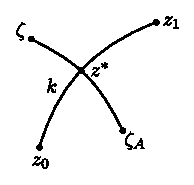
\includegraphics{vol29-fig/fig29-10.eps}
\smallskip
\caption{}
\label{chap1:fig10}
\end{figure}

Then $k$ is an edge of $\mathfrak{F}_A$ and therefore $A^{-1}<k>$ is
an edge of $\mathfrak{F}$. If $A^{-1}<k>=k$, then $A^{-1}$ permutes
$z_0$ and \pageoriginale $z_l$, since $A^{-1}$ preserves the
orientation. It follows now that $A^2=\pm E$. Since $A^{-1}$ permutes
$\zeta$ and $\zeta_A$ also, the two lines $\widehat{\zeta\zeta_A}$ and
$\widehat{z_0z_1}$ are mapped onto themselves and therefore the point
of intersection $z^{\ast}$ of these two lines must be a fixed point of
$A$. Hence $A$ is an elliptic transformation of order 2. We introduce
$z^{\ast}$ as a vertex of $\mathfrak{F}$. Then the two edges
$\widehat{z_0z^{\ast}}$ and $\widehat{z^{\ast}z_1}$ are permuted by
$A$. If $A^{-1}<k> \neq k$, then we have an edge of $\mathfrak{F}$
different from $k$ but equivalent to $k$ by $\Gamma$. proceeding in
this way, we obtain that $\mathfrak{F}$ is a closed convex polygon
bounded by a finite number of hyperbolic straight lines $k_i,
k^{\ast}_i (i=1,2,\ldots t)$ such that $k_i$ and $k^{\ast}_i$ are
pairwise equivalent under $\Gamma$ i.e. there exist elements $A_i
\in \Gamma$ such that $A_i <k^{\ast}_i>= k_i(i=1,2,\ldots ,
t)$. We shall call the transformations $A_i$ \textit{the boundary
  substitutions of } $\mathfrak{F}$. For a given $\mathfrak{F}$, if
$\{A_i | i = 1, 2, \ldots, t\}$ is a set of its boundary
substitutions, then the set $\{A^{\pm 1}_i, i = 1, 2, \ldots, t\}$ is
uniquely determined by $\mathfrak{F}$.

We shall see that the set of boundary substitutions of the fundamental
domain $\mathfrak{F}$ generate the group $\Gamma$. First, we prove the
following 
\end{proof}

\begin{lem}\label{chap1:lem2}
Let $\mathfrak{F}$ be a normal fundamental domain of a discrete group
$\Gamma$ of transformations of the hyperbolic plane. Then any compact
set $K$ in the hyperbolic plane has non-empty intersection with only a
finite number of images of $\mathfrak{F}$ under elements of $\Gamma$.
\end{lem}

\begin{proof}
Without loss of generality, we can assume that $K$ is a disc with
centre $\zeta$ and radius $\rho$. If possible, let $\mathfrak{F}_{S_i}
\cap K \neq \phi$ for an infinity of distinct $S_i (\in
\Gamma), i=1,2,\ldots$ Picking $z^{(i)}$ in $\mathfrak{F}_{S_i} \cap
K$, we have $z^{(i)}_{S^{-1}_i}\in \mathfrak{F}$ and 
$$
\delta(z^{(i)},\zeta) \leq \rho \Longrightarrow \rho >
\delta\left(z^{(i)}_{S^{-1}_i}, \zeta_{S^{-1}_i}  \right) \geq \delta
\left(z^{(i)}_{S^{-1}_i },\zeta\right).
$$\pageoriginale

Therefore
$$
\delta (\zeta,\zeta_{S_i}) \leq \delta (\zeta,z^{(i)}) + \delta
(z^{(i)}, \zeta_{S_i}) \leq \rho + \rho = 2\rho,
\text{ for } i = 1,2,3, \ldots 
$$
which is impossible from the discreteness of $\Gamma$. The proof of
the lemma is complete. 
\end{proof}

\begin{thm}\label{chap1:thm5}
The set of the boundary substitutions of a normal fundamental domain
for a discrete group $\Gamma$ of transformations of the hyperbolic
plane generates $\Gamma$.
\end{thm}

\begin{proof}
Let $\mathfrak{F}$ be a normal fundamental domain for $\Gamma$ with
the centre $\zeta$. Let $S$ be an arbitrary element of $\Gamma$. Then
by Lemma 2, the hyperbolic straight line $\widehat{\zeta\zeta_S}$
intersects only a finite number of images of $\mathfrak{F}$ under
elements of $\Gamma$. Let $\mathfrak{F}_{B_0},\mathfrak{F}_{B_1},
\ldots, \mathfrak{F}_{B_n}$ be the images of $\mathfrak{F}$, which
intersect $\widehat{\zeta\zeta_S}$ and are so arranged that
$\mathfrak{F}_{B_{i-1}}$ and $\mathfrak{F}_{B_i}$ have an edge, say
$s_i$, in common. Then $B_0= \pm E$ and $B_n= \pm S$. Obviously,
$B^{-1}_{i-1}(s_i)$ is an edge of $\mathfrak{F}$ and it is the
perpendicular bisector of $\widehat{\zeta\zeta}_{B^{-1}_{i-1}B_i}$; therefore,
we must have $B^{-1}_{i-1}B_i = \pm A^{\pm 1}_{r i}$, where $A_{r_i}$
is a boundary substitution of $\mathfrak{F}$. It is now immediate that
$s=\pm B_0 B_1B^{-1}_1 B_2B^{-1}_2 B_3 \ldots B^{-1}_{n-1} B_n =\pm
A^{\pm 1}_{r_1} \ldots A^{\pm 1}_{r_n}$ and our theorem is proved. 

Let $d(U)$ denote the Euclidean diameter of an arbitrary point set
$U$. We now show that for $\in > 0$, $d(\mathfrak{F}_A)\leq
\in$ for almost all $A$ in $\Gamma$. By Lemma~\ref{chap1:lem2},
\pageoriginale only finitely many images of $\mathfrak{F}$ intersect
the circle $\{z||z|\leq h < 1\}$. Let $\mathfrak{F}_A$ with $A$ in
$\Gamma$ be outside the disc $|z|\leq h$.

\begin{figure}[H]
\centering
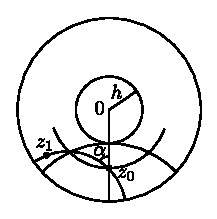
\includegraphics{vol29-fig/fig29-11.eps}
\smallskip
\caption{}
\label{chap1:fig11}
\end{figure}

Choose $z_0 \in \mathfrak{F}_A$ so that $|z_0| =
\inf\limits_{z\in \mathfrak{F}_A}(|z|)$. Then the hyperbolic tangent
to $|z|=h$ at the point of intersection of $|z|=h$ and the line
joining $0$ and $z_0$ is perpendicular to this line. We claim that
$\mathfrak{F}_A$ lies in the lens domain bounded by the hyperbolic
tangent mentioned above and the unit circle, which is also defined by 
$$
\left| z - \frac{z_0}{|z_0|} \frac{1+h^2}{2h}\right| \leq
\frac{1-h^2}{2h}, |z| \leq 1.
$$

If possible, let $z_1 \in \mathfrak{F}_A$ lie outside the
above lens domain; then the line $\widehat{z_0z_1}$ is in
$\mathfrak{F}_A$, because $\mathfrak{F}_A$ is a convex set. But the
angle $\alpha$ (see Figure~\ref{chap1:fig11} is $<\pi/2$; therefore, there exists a
point $z^{\ast}$ on the hyperbolic line $\widehat{z_0z_1}$ such that
$|z^{\ast}|<|z_0|$, which contradicts the minimality of $|z_0|$. Hence
$\mathfrak{F}_A$ lies in the above lens domain. It can be seen easily
that the diameter of this domain is $2(1-h^2)/(1+h^2)$. Therefore it
follows that 
$$
d(\mathfrak{F}_A) < 2 (1-h^2)/(1+h^2) \to 0 \text{ as } h \to 1.
$$

We now assert that a discrete group $\Gamma$ with a normal fundamental
domain of finite area is a \textit{Grenzkreis group of the first kind}
in the sense of Petersson \pageoriginale \cite{c1:key3}. In order to prove
this assertion, we have to show that, given a point $z^{\ast}$ with
$|z^{\ast}|=1$, there exists a sequence of points $z_n$ in
$\mathfrak{L}$ and a sequence $\{L_n\}$ of pairwise distinct
transformations $L_n \in \Gamma$ such that 
$$
\lim\limits_{n\to \infty} z_n = \lim\limits_{n\to \infty} L_n <z_n> =
z^{\ast}. 
$$

For given $\in >0, n-1$ elements $S_1, S_2, S_3,\ldots \ldots,
S_{n-1}$ in $\Gamma$ and a point $z^{\ast}$ with $|z^{\ast}|=1$, we
can find $S$ in $\Gamma$ with $S\neq S_i, i=1,2,\ldots, n-1$ and a
point $z$ in $|z|<1$ such that 
$$
|z-z^{\ast}| < \in, |z_S-z^{\ast}| < 2\in. 
$$

In order to prove this, we consider the point set
$$
U_{\in} = \{z||z-z^{\ast}|<\in, |z|<1\}.
$$

Since $\mathfrak{I} (U_{\in}) = \infty$, infinitely many
images $\mathfrak{F}_T$ will intersect $U_{\in}$. Therefore,
we have $U_{\in} \cap \mathfrak{F}_T \neq \emptyset$ for infinitely
many $T$ and $d(\mathfrak{F}_T) < \in$, for almost all $T$.

Let $T_1$ and $T_2$ be two elements of $\Gamma$ satisfying the above
two conditions and the additional condition
$$
T_2 \neq S_i T_1 \text{ for } i = 1, 2, \ldots , n-1.
$$

We choose a point $z\in \mathfrak{F}_{T_1} \cap
U_{\in}$ and set $S=T_2 T^{-l}_1$ so that $S<z>\in
\mathfrak{F}_{T_2}$. Let $z'$ be a point in $U_{\in} \cap
  \mathfrak{F}_{T_2}$. Then $|z'-z^{\ast}|<\in$ and
  $|z'-z_S|<\in$. This shows that 
$$
|z^{\ast} - z_S|\leq |z^{\ast} - z'| + |z'-z_S| \leq 2 \in.
$$

But \pageoriginale since $z$ belongs to $U_{\in}$,
$|z-z^{\ast}|<\in$; therefore $z$ chosen above is a required
point. Let $\in =\dfrac{1}{n}, z=z_n$ and $S= S_n$. Then
obviously the sequences $\{z_n\}$ and $\{S_n <z_n>\}$ converge to
$z^{\ast}$ as $n\to \infty$. Moreover, by choice, the elements of the
sequence $\{S_n\}$ are pairwise distinct. This completely proves our
assertion that $\Gamma$ is a Grenzkreis group of the first kind.

We mention only the validity of the converse fo the above statement,
namely: a Grenzkreis group of the first kind has a normal fundamental
domain $\mathfrak{F}$ with finite area. This assertion amounts
essentially to the statement that $\mathfrak{F}$ is bounded by a finite
number of line segments which lie on hyperbolic straight lines. This
was proved by M. Heins, W. Fenchel and J. Nielsen (jointly),
L. Greenberg, A. Marden (cf. the article of L. Greenberg in ``Discrete
Groups and Automorphic Functions'', edited by W.J. Harvey, Academic
Press 1977, and the cited literature).

Following Rankin \cite{c1:key6}, we call a discrete group with a normal
fundamental domain of finite area a \textit{horocyclic group}. The
boundary of a normal fundamental domain for a discrete group can be
described by means of the so-called \textit{isometric circles of the
  group} discussed by Ford \cite{c1:key1}.
\end{proof}

\section{Riemann surfaces}\label{chap1:sec4}%%% 4
Let $\mathfrak{F}$ be a closed normal fundamental domain for a
horocyclic group $\Gamma$. Let $\zeta$ be the centre of
$\mathfrak{F}$. By joining $\zeta$ with the vertices of
$\mathfrak{F}$, we \pageoriginale obtain a decomposition of
$\mathfrak{F}$ into an even number of triangles. If we identify the
equivalent edges of $\mathfrak{F}$, we get a closed orientable
polyhedron $\mathscr{R}$. Let $p$ denote the topological genus of
$\mathscr{R}$. If $e,k$ and $d$ denote respectively the number of
vertices, the number of edges and the number of triangles of
$\mathscr{R}$, then the Euler-Poincare characteristic formula states
that 
$$
e-k+d=2-2p.
$$

Let $\mathfrak{g}_1, \mathfrak{g}_2, \ldots \mathfrak{g}_{\sigma}$ be the
different classes of parabolic cusps and $\mathfrak{n}_1,\break
\mathfrak{n}_2, \ldots , \mathfrak{n}_{e_1}$ be the classes of the
proper cusps of $\mathfrak{F}$. Let $z_{i1}, z_{i2}, \ldots,
z_{ir_{i}}$ be all the vertices of $\mathfrak{F}$ in the class
$\mathfrak{n}_i$ and $\omega^{(1)}_i, \omega^{(2)}_i, \ldots
,\omega^{(r_i)}_i$ be the angles of $\mathfrak{F}$ at the vertices
$z_{ij}$, $j=1,2,\ldots, r_i$. Then 
$$ 
\omega^{(1)}_i + \omega^{(2)}_i + \cdots + \omega^{(r_i)}_i = 2
\pi/\ell_i \;\; (i = 1, 2, \ldots e_1)
$$
for some natural number $\ell_i$. We have already proved that $z_{ij}$
for $j=1,2, \ldots ,r_i$ are fixed points of elliptic transformations
in case $\ell_i >1$ and the group of transformations which leave
$z_{ij}$ fixed is of order $\ell_i$. Since, for a fixed $i$, the two
points $z_{ij}$ and $z_{ij'}$ for $j \neq j'$ are equivalent, the
groups leaving $z_{ij}$ and $z_{ij'}$ fixed are conjugate subgroups of
$\Gamma$. Let $e_0$ be the number of classes of proper cusps of
$\mathfrak{F}$ for which $\ell_i >1$. We so choose our notation that 
$$
\ell_i > 1 \text{ for } i = 1,2, \ldots, e_0.
$$

It is obvious that the sum of the angles of all the triangles of
$\mathscr{R}$ is given by \pageoriginale
$$
2 \pi  + \sum^{e_1}_{i=1} \{\omega^{(1)}_i + \omega^{(2)}_i + \cdots + 
\omega^{(r_{i})}_i\} = \pi d - \mathfrak{I} (\mathfrak{F}).
$$
and consequently
$$
1 + \sum^{e_1}_{i=1} 1/\ell_i = \frac{1}{2} d -\frac{1}{2\pi} 
\mathfrak{I} (\mathfrak{F}). 
$$

Obviously, we have $e=\sigma + e_1 + 1$. Since each edge belongs
exactly to two triangles, we have $3d = 2k$. As a result, $\sigma +
e_1 + 2 p =\dfrac{1}{2}d+1$ and therefore 
\begin{align*}
\sigma + e_1 + 2p & = 2 + \sum^{e_1}_{i=1} 1/\ell_i + \frac{1}{2\pi}
\mathfrak{I} (\mathfrak{F}); \\
\text{i.e. } \quad\frac{1}{2\pi} \mathfrak{I} (\mathfrak{F})
& = 2p - 2 + \sigma + e_1 - \sum^{e_1}_{i=1} 1/\ell_i\\
& = 2p - 2 + \sigma + \sum^{e_0}_{i=1} (1-1/\ell_i), \tag{1}\label{eq4:1}
\end{align*}
since $\ell_i = 1$ for $e_0 < i \leq e_1$.

It can be shown easily that the right hand side of equation (1) has a
positive minimum equal to $1/42$. This minimum is attained only
for one set of values, namely, $p=0$, $\sigma=0$, $e_0=3$, $\ell_1=2$,
$\ell_2=3$ and $\ell_3 = 7$. It can be proved that there exists a
group for which a fundamental domain has area $\pi/21$. (For the
proof, see \cite{c1:key2}, page 621). Thus, in general, 
$$
\mathfrak{I} (\mathfrak{F}) \geq \pi / 21,
$$
where $\mathfrak{F}$ is a fundamental domain for a horocyclic
group. For $\sigma >0$, the right hand side of \eqref{eq4:1} has the minimum
$1/6$ and therefore, in this case, $\mathfrak{I}(\mathfrak{F}) \geq
\pi/3$. This minimum is again attained for only one set of values
given \pageoriginale by $p=0$, $\sigma=1$, $e_0 = 2$, $\ell_1=2$ and
$\ell_2 =3$. We shall see later that this set of values is realised
for `the modular group'.

We now prove that the area of a normal fundamental domain for a
horocyclic group does not depend on the choice of its centre
$\zeta$. Assume that $\mathfrak{g}$ is a fundamental domain for
$\Gamma$ bounded by only a finite number of segments of hyperbolic
straight lines. Then we conclude that 
$$
z \in \mathfrak{F} \Longrightarrow z_A \in
\mathfrak{g} \text{ for some } A \in \Gamma \Longrightarrow z
\in \mathfrak{g}_{a^{-1}} \cap \mathfrak{F}
$$
or
$$
\bigcup_{\pm A \in \Gamma} (\mathfrak{g}_{A^{-1}} \cap
\mathfrak{F}) = \mathfrak{F}.
$$

The sets $\mathfrak{g}_{A^{-1}}\cap \mathfrak{F}$ and
$\mathfrak{g}_{B^{-1}} \cap \mathfrak{F}$ intersect on their common
boundary for $B\neq \pm A$. For, $z\in (\mathfrak{g}_{A^{-1}}
\cap \mathfrak{F}) \cap (\mathfrak{g}_{B^{-1}} \cap \mathfrak{F})$
implies that $z_A$ and $z_B$ belong to the boundary of $\mathscr{G}$
i.e. $z$ is a boundary point of $\mathfrak{g}_{A^{-1}}$ and
$\mathfrak{g}_{B^{-1}}$ and therefore of the sets $\mathfrak{g}_{A^{-1}}
\cap \mathfrak{F}$ and $\mathfrak{g}_{B^{-1}} \cap \mathfrak{F}$. Since
the sets $\mathfrak{g}_{A^{-1}} \cap \mathfrak{F}$ for $A\in
\Gamma$ are measurable and the intersection of two such distinct sets
is a set of measure zero, we have
$$
\mathfrak{I} (\mathfrak{F}) = \sum_{\pm A \in \Gamma}
\mathfrak{I} (\mathfrak{g}_{A^{-1}} \cap \mathfrak{F}) = \sum_{\pm A
  \in \Gamma} \mathfrak{I} (\mathfrak{G} \cap\mathfrak{F}_A) =
\mathfrak{I} (\mathfrak{G})
$$
and our assertion is completely proved.

It can be shown that the polyhedron $\mathscr{R}$ is topologically
equivalent to the space obtained by adding to the quotient-space
$\mathfrak{H}/\Gamma$ the equivalence classes of parabolic cusps which
are sufficient to compactify the space $\mathfrak{g}/\Gamma$, provided
the neighbourhoods of the cusps are defined in a suitable way. 

In the \pageoriginale following, we shall speak of
$\overline{\mathfrak{H}} = \mathfrak{H} \cup$ \{all parabolic cusps of
$\Gamma$\} as a covering surface of $\mathscr{R}$. Let
$\mathfrak{g}\in \mathscr{R}$; we say that $\mathfrak{g}$ is
\textit{the trace point} of $\tau \in \mathfrak{g}$ if $\tau$
belongs to $\overline{\mathfrak{H}}$.

\begin{defi*}
An equivalence class $\mathfrak{g} \in \mathscr{R}$ of
parabolic cusps is called a \textit{logarithmic branch point}.
\end{defi*}

Thus the number of logarithmic branch points of $\mathscr{R}$ is $\sigma$.

\begin{defi*}
Let $\mathfrak{g} \in \mathscr{R}$ be the trace point of
$\tau_0 \in \mathfrak{H}$. Then, for $-E\in \Gamma,
\overline{\Gamma}_0= \Gamma_0|\{\pm E\}$ where $\Gamma_0 =
\{S|S<\tau_0> = \tau_0, S \in \Gamma\}$, is a cyclic group of
order $\ell$ uniquely determined by $\mathfrak{g}$. We shall call
$\mathfrak{g}$ a \textit{branch point of $\mathscr{R}$ of order} $\ell
- 1$ or a point $\tau_0 \in \mathfrak{g}$ a point of
\textit{ramification index} $\ell-1$ if $\ell>1$. If $\ell=1$, we
shall call $\mathfrak{g}$ a \textit{reqular point} of $\mathscr{R}$.
\end{defi*}

We have already observed that there exist only finitely many branch
points of $\mathscr{R}$. Therefore, given a branch point $\mathfrak{g}$
of $\mathscr{R}$, there exists a neighbourhood of $\mathfrak{g}$ which
does not contain any other branch point of $\mathscr{R}$.

We shall now introduce some \textit{local uniformising parameters} or,
as we shall usually say, \textit{local coordinates} on $\mathscr{R}$
which define an analytic structure on $\mathscr{R}$ for which it is a
Riemann surface. We shall call $\mathscr{R}$ the \textit{Riemann
surface associated to the group} $\Gamma$. A \textit{local
coordinate at a point} $\mathfrak{g}_0$ of $\mathscr{R}$ is a
function $t(\mathfrak{g})$ such that 
\begin{itemize}
\item[1)] $t(\mathfrak{g})$ maps topologically an open
  neighbourhood $U_0$ of $\mathfrak{g}_0$ onto an open neighbourhood of
  $0$ in the complex $t$-plane,

\item[2)] for another point $\mathcal{G}$ of $U_0$, $t-t(\mathcal{G})$
  is a local coordinate at $\mathcal{G}$, and 

\item[3)] if $s=s(\mathfrak{g})$\pageoriginale is another local
  coordinate at $\mathfrak{g}_0$, then in a neighbourhood of
  $\mathfrak{g}_0$, the function $s$ can be expressed as a convergent
  power series 
$$
s=c_1 t + c_2 t^2 + \ldots \text{ with } c_1 \neq 0
$$
and conversely, every such convergent power series defines a local
coordinate at $\mathfrak{g}_0$.
\end{itemize}

Let $g(\mathfrak{g})$ be a function defined in a neighbourhood of
$\mathfrak{g}_0$ such that 
$$
g(\mathfrak{g}) = \sum^{\infty}_{r=k} c_r t^r, c_k \neq 0,
$$
where $t=t(\mathfrak{g})$ is a local coordinate at
$\mathfrak{g}_0$. Then $g(\mathfrak{g})$ is said to be of
\textit{degree} $k$ at $\mathfrak{g}_0$. It can be verified that $k$
does not depend upon the choice of a local coordinate at
$\mathfrak{g}_0$. If $k \geq 0$, then $g(\mathfrak{g})$ is said to be
\textit{regular at} $\mathfrak{g}_0$. We call $\mathfrak{g}_0$ a
\textit{zero of order} $k$ of $g(\mathfrak{g})$ when $k>0$ and a
\textit{pole of order} $|k|$ when $k<0$.

In what follows, by a domain we shall always understand an open
connected set.

\begin{defi*}
Let $\mathcal{G}^{\ast}$ be a domain in $\overline{\mathfrak{H}}$. A
function $f(\tau)$ defined in $\mathcal{G}^{\ast}$ is said to be an
\textit{automorphic function with respect to a horocyclic group}
$\Gamma$, if 
$$
f(\tau_S) = f(\tau) \text{ for } S \in \Gamma, \text{ whenever
} \tau \text{ and } \tau_S \text{ are in } \mathcal{G}^{\ast}.
$$
\end{defi*}

Now $\mathcal{G} = \{\mathfrak{g}|\mathfrak{g} \in
\mathscr{R}, \mathfrak{g}$ is the trace point of some $\tau$ in
$\mathcal{G}^{\ast}$\} is a domain in $\mathscr{R}$ and the function
$g(\mathfrak{g})$ defined by $g(\mathfrak{g}) = f(\tau)$, where
$\mathfrak{g}$ is the trace point of $\tau$, is well-defined in
$\mathcal{G}$. Conversely, let $\mathcal{G}$ be a domain
\pageoriginale in $\mathscr{R}$, $\mathcal{G}^{\ast}=\{\tau|\tau
\in \overline{\mathfrak{H}}$, the trace point of $\tau$
belongs to $\mathcal{G}$\} and $\mathcal{G}^{\ast}_0$ a connected
component of $\mathcal{G}^{\ast}$. If $g(\mathfrak{g})$ is a function
defined in $\mathcal{G}$, then the function $f(\tau)$ defined by
$f(\tau)=g(\mathfrak{g})$, where $\mathfrak{g}$ is the trace point of
$\tau$, is an automorphic function defined in $\mathcal{G}^{\ast}_0$
with respect to $\Gamma$. 

We now describe a suitable system of local coordinates at various
points of $\mathscr{R}$.
\begin{enumerate}
\item Let $\mathfrak{g}_0 \in \mathscr{R}$ be a branch point
  of order $\ell-1$. Let $\tau_0$ be a point in $\mathfrak{H}$ with
  the trace point $\mathfrak{g}_0$. Then the subgroup
  $\overline{\Gamma}_0 \subset \overline{\Gamma}(=\Gamma$ modulo
  $\{\pm E\}$, if $-E\in \Gamma$) consisting of those
  transformations of $\overline{\Gamma}$ which leave $\tau_0$ fixed is
  a cyclic group of order $\ell$. Let $L$ be a generator of
  $\overline{\Gamma}_0$, which we can take to be a rotation through an
  angle $2\pi/\ell$. Defining $z$ by
  $z=(\tau-\tau_0)/(\tau-\bar{\tau}_0)$, the transformation $\tau \to
  \tau_L$ corresponds to the mapping $z\to e^{2\pi
    i/\ell}z$. Actually, we have, for $L=\left(\begin{smallmatrix}
  a&b\\c&d\end{smallmatrix} \right)$,
$$
\frac{L<\tau>-\tau_0}{L<\tau>-\overline{\tau}_0} = 
\frac{L<\tau>-L<\tau_0>}{L<\tau>-L<\overline{\tau}_0>} = 
\frac{c\overline{\tau}_0 + d}{c\tau_0 + d} \cdot \frac{\tau -
\tau_0}{\tau-\overline{\tau}_0} = \mu
\frac{\tau-\tau_0}{\tau-\overline{\tau}_0},  
$$
where $|\mu|=1$. If $U=\{ \tau \in
\mathfrak{H}\arrowvert|z|<\in\}$ is an open disc with centre
$\tau_0$ and with $\in$ small enough to ensure that the
equivalence of $\tau_{1}$ and $\tau_2$ in $U$ under
$\overline{\Gamma}$ implies already their equivalence under
$\overline{\Gamma}_0$, then, only for $\tau=\tau_0$, a point $\tau$
in $U$ is uniquely determined by its trace point $\mathscr{g}$. For
$\tau \neq \tau_0$ in $U$, there exist exactly $\ell$ different points
$\tau_1, \tau_2, \ldots , \tau_{\ell}$ with the same trace point
$\mathfrak{g}$ as $\tau$. But precisely one of these $\ell$ points
belongs to $U_0 = \{\tau \in U\arrowvert |z|<\in, 0
\leq arg z < 2 \pi/\ell\}$. This $\tau \to \mathfrak{g}$ is a $1-1$
mapping of $U_0$ onto a neighbourhood of $\mathfrak{g}_0$ in
$\mathscr{R}$. Moreover, $z\to t = z^{\ell}$ is a 1-1 mapping of $U_0$
onto the open disc $\{t\arrowvert |t| <
\in^{\ell}\}$. Finally, $\mathfrak{g} \to \tau \to t$ is a 
1-1 mapping, \pageoriginale via $U_0$, of a neigbourhood of
$\mathfrak{g}_0$ on $\mathscr{R}$ onto a neighbourhood of 0 in the
complex plane. Let us assume that there exists an analytic structure
on $\mathscr{R}$ such that $t$ is regular at $\mathfrak{g}_0$ with
respect to this analytic structure. Then 
$$
t = c_0 + c_1 s + c_2 s^2+ \cdots,
$$
where $s=s(\mathfrak{g})$ is a local coordinate at
$\mathfrak{g}_0$. But $t(\mathfrak{g}_0)=s(\mathfrak{g}_0)=0$ and
$s\to t$ is $a$ 1-1 map, therefore $c_0=0$ and $c_1\neq 0$. This
shows that $t$ is necessarily a local coordinate at $\mathfrak{g}_0$.

\item Let $\mathfrak{g}_0$ be a logarithmic branch point of
  $\mathscr{R}$, $\tau_0$ a parabolic cusp with trace point
  $\mathfrak{g}_0$ and $A$ a transformation of $\mathfrak{H}$ onto
  itself which maps $\tau_0$ to $\infty$. Thus the group $A\Gamma
  A^{-1}$ has $\infty$ as a parabolic cusp. The subgroup
  $\overline{\Gamma}_0 \subset \Gamma / \{\pm E\}$, consisting of
  those transformations leaving $\tau_0$ fixed is an infinite cyclic
  group generated by some transformation, say $P$. Setting
  $\tau_{\ast} = A<\tau>$, the transformation $\tau  \to \tau_P$
  corresponds to a translation $\tau^{\ast} \to \tau^{\ast}+ \mu$,
  where we can assume that $\mu >0$. We introduce $U_0=\{\tau |
  \tau^{\ast} = x^{\ast} + iy^{\ast}, 0 \leq x^{\ast} < \mu , y^{\ast}
  > m\}$ and conclude, as in the preceding case, that, for large enough
  $m$, the mapping $\mathfrak{g} \to \tau \to t =e^{2\pi i A
  <\tau>/\mu}(\tau\in U_0)$ for $\mathfrak{g}\neq
  \mathfrak{g}_0$, together with $\mathfrak{g}_0 \to \tau_0 \to 0$
  gives a 1-1 mapping of a neighbourhood of $\mathfrak{g}_0$ onto a
  neighbourhood of 0 in the complex plane. The assumption about $t$
  being regular at $\mathfrak{g}_0$ with respect to a given analytic
  structure on $\mathscr{R}$ implies again that $t(\mathfrak{g})$ is
  necessarily a local coordinate at $\mathfrak{g}_0$.

It \pageoriginale can be checked that the local coordinate system on
$\mathscr{R}$ that we have defined in (i) and (ii) above has all the
properties required of a local coordinate system on $\mathscr{R}$.

Let $f(\mathfrak{g})$ be a meromorphic function defined in a
neighbourhood of $\mathfrak{g}_0$ and of degree $k$. Then
$f(\mathfrak{g})$ has a power-series expansion
$$
f(\mathfrak{g}) = \sum^{\infty}_{n=k} c_n t^n \text{ with } c_k \neq 0,
$$
where $t=((\tau -\tau_0)/(\tau-\overline{\tau}_0))^{\ell}$ or $e^{2\pi
i A <\tau>/\mu}$ according as $\mathfrak{g}_0$ is a branch point of
order $\ell-1$ or a logarithmic branch point.
\end{enumerate}

\section{Meromorphic functions and Differentials}\label{chap1:sec5}%%% 5

In this section, $\Gamma$ will denote a horocyclic group and
$\mathscr{R}$ the Riemann surface associated to $\Gamma$.

\begin{defi*}
A function $f(\mathfrak{g})$ defined in a domain $\mathcal{G}$ of
$\mathscr{R}$ is said to be a meromorphic function on $\mathcal{G}$
if, for every point $\mathfrak{g}_0 \in \mathcal{G}$, the
function has a power series expansion, in terms of a local coordinate
at $\mathfrak{g}_0$, with only a finite number of negative exponents.
\end{defi*}

If $f(\mathfrak{g})$ is defined on the whole of $\mathscr{R}$, then it
will have at most a finite number of poles because $\mathscr{R}$ is
compact; otherwise, $f(\mathfrak{g})$ can have an infinite number of
poles in the domain of its definition. The set of all meromorphic
functions on $\mathscr{R}$ forms a field. A meromorphic function
$f(\mathfrak{g})$ on $\mathscr{R}$ gives rise to an \pageoriginale
automorphic function $f(\tau)$ on $\mathfrak{H}$ for the group
$\Gamma$ with $f$ meromorphic on $\mathfrak{H}$ and having a Fourier
expansion 
$$
f(\tau) = \sum^{\infty}_{n-k} c_n e^{2\pi \text{ in } A <\tau>/\mu},
c_k \neq 0.
$$
at a parabolic cusp $\tau_0$ of $\Gamma$, where $A$ denotes a
transformation of $\mathfrak{H}$ on to itself mapping the cusp
$\tau_0$ to $\infty$. Conversely, it is obvious that every such
automorphic function on $\mathfrak{H}$ defines a meromorphic function
on $\mathscr{R}$. In the following, we shall denote by
$v_{\mathfrak{g}}(f)$ the degree of the meromorphic function
$f(\mathfrak{g})$ at the point $\mathfrak{g}$ belonging to the domain
of definition of $f$. We shall call the product $\prod\limits_{\mathfrak{g}}
\mathfrak{g}^{v_{\mathfrak{g}}(f)}$ \textit{the divisor of $f$} and
the sum $\sum\limits_{\mathfrak{g}} v_{\mathfrak{g}}(f)$ \textit{the degree
  of $f$ on} $\mathscr{R}$ and denote them by $(f)$ and $v(f)$
respectively. Since $f(\mathfrak{g})$ can have only a finite number of
zeros and poles on $\mathscr{R}$, the product $(f)$ is a finite
product and the sum $v(f)$ is finite.

\begin{defi*}
Let $\mathcal{G}$ be a domain in $\mathscr{R}$. A \textit{meromorphic
differential} or simply \textit{a differential} $\omega$ on
$\mathcal{G}$ is an assignment, for every local coordinate $t$ in
$\mathcal{G}$, of a meromorphic function $\omega_t$ defined in the
domain of definition of $t$ such that the following condition is
satisfied:
\end{defi*}

It $t$ and $s$ are two local coordinates defined in $\mathcal{G}$ with
$U_t$ and $U_s$ as their domain of definition, then 
$$
\omega_s \frac{ds}{dt} = \omega_t \text{ in } U_t \cap U_s.
$$

Two differentials $\omega$ and $\omega^{\ast}$ on $\mathcal{G}$ are
equal, whenever $\omega_t = \omega^{\ast}_t$ for every local
coordinate $t$ defined in $\mathcal{G}$. Using the condition in the
definition of a differential, it can be shown, by means of the
principle of analytic continuation, that two differentials $\omega$
and $\omega^{\ast}$ are equal, if $\omega_t=\omega^{\ast}_t$
holds \pageoriginale for some one local coordinate $t$. If
$f(\mathfrak{g})$ is a meromorphic function defined on $\mathcal{G}$,
then it defines on $\mathcal{G}$ a meromorphic differential $df$ for
which $(df)_t=\dfrac{df}{dt}$. If $\omega$ is a differential and
$f(\mathfrak{g})$ a meromorphic function on $\mathcal{G}$, then by
$f_{\omega}$ we shall understand the differential which assigns the
meromorphic function $f\omega_t$ to the local variable $t$ defined in
$\mathcal{G}$. It follows that if $\omega$ is a differential defined
in $\mathcal{G}$, then $\omega=\omega_tdt$; for,
$$
(\omega_t dt)_t = \omega_t \frac{dt}{dt} = \omega_t.
$$

Thus if $t$ is a local coordinate at a point $\mathfrak{g}_0$ of
$\mathcal{G}$, then 
$$
\omega = \omega_t dt = \left(\sum^{\infty}_{n=k} c_n t^n\right) dt.
$$

We define the \textit{degree of} $\omega$ at $\mathfrak{g}_0$ to be
the least $k$ for which $c_k \neq 0$ and denote it by
$v_{\mathfrak{g}_0}(\omega)$. It can be seen easily that the degree of
a differential at a point does not depend upon the choice of the local
coordinate at the point. We say that $\mathfrak{g}_0$ is a
\textit{zero or a pole of} $\omega$, if it is a zero or a pole of
$\omega_t$. If $\omega$ is a meromorphic differential on
$\mathscr{R}$, we define the \textit{divisor $(\omega)$ and degree}
$v(\omega)$ in the same way as we defined the divisor and degree of a
meromorphic function on $\mathscr{R}$ i.e. $(\omega) =
\prod\limits_{\mathfrak{g}} \mathfrak{g}^{v_{\mathfrak{g}}(\omega)}$ and
$v(\omega) = \sum\limits_{\mathfrak{g}} v_{\mathfrak{g}}(\omega)$. We shall
call the coefficient $c_{-1} (c_{-1}= 0$ if $k\geq 0$) in the
expansion of $\omega$ at $\mathfrak{g}_0$ mentioned above as the
\textit{residue} of $\omega$ at $\mathfrak{g}_0$ and write 
$$
\text{res}_{\mathfrak{g}_0} \omega = c_{-1}.
$$

The independence of the residue of $\omega$ at $\mathfrak{g}_0$ from
the choice of $t$ follows \pageoriginale from the integral
representation for the residue given by 
$$
c_{-1} = \frac{1}{2\pi i} \oint \omega_t \; dt, 
$$
where the integral is over a closed curve winding round 0 exactly
once and contained in the domain of definition of $t$.

Let $\omega$ be a differential on $\mathscr{R}$. We say that 
\begin{itemize}
\item[1)] $\omega$ is of \textit{the first kind}, if
  $v_{\mathfrak{g}}(\omega)\geq 0$ for every $\mathfrak{g}\in
  \mathscr{R}$, 

\item[2)] $\omega$ is of \textit{the second kind}, if $\omega$ has at
  least one pole and the residues at the various poles vanish, and 

\item[3)] $\omega$ is of \textit{the third kind}, if $\omega$ is not
  any of the above two kinds i.e. $\omega$ has at least one pole with
  a non-zero residue.
\end{itemize}

Let $\mathfrak{g}_0$ be the trace point of $\tau_0\in
\mathfrak{H}$ and let further, $\mathfrak{g}_0$ be a regular
point. Then $\tau-\tau_0$ and $S<\tau>-S<\tau_0>$ for $S\in
\Gamma$ are local coordinates at $\mathfrak{g}_0$. If $\omega$ is a
differential on $\mathscr{R}$, then 
$$
\omega_{(\tau-\tau_0)} = \omega_{(S<\tau>-S<\tau_0>)} (c\tau + d)^{-2},
\text{ where } S = \left(\begin{smallmatrix}
a&b\\c&d\end{smallmatrix} \right).
$$

For, by definition of $\omega$, we have 
\begin{align*}
\omega_{(\tau-\tau_0)} & = \omega_{(S<\tau>-S<\tau_0>)}
\frac{d(S<\tau>-S<\tau_0>)}{d(\tau -\tau_0)}\\
& = \omega_{(S<\tau>-S<\tau_0>)} (c\tau + d)^{-2}.
\end{align*}

Moreover, if $\tau_1$ is another point such that the trace point
$\mathfrak{g}_1$ of $\tau_1$ lies `sufficiently near'
$\mathfrak{g}_0$, then $\mathfrak{g}_1$ is a regular point and
$\tau-\tau_1$ is a local \pageoriginale coordinate at
$\mathfrak{g}_1$. Therefore, we have 
$$
\omega_{(\tau-\tau_0)} = \omega_{\tau-\tau_1} \frac{d(\tau-\tau_1)}{dt}
dt = \omega_{(\tau-\tau_1)}
$$
showing that $\omega_{(\tau-\tau_0)}$ is independent of the choice of
$\tau_0$ in a neighbourhood of $\tau_0$. But if $\tau_1$ is not
`sufficiently near' $\tau_0$, then we can join them by a curve which
does not pass through the parabolic and elliptic fixed points of
$\Gamma$; it can then be seen easily that $\omega_{(\tau-\tau_1)}$ can
be obtained by analytic continuation of $\omega_{(\tau-\tau_0)}$ along
the curve joining $\tau_0$ and $\tau_1$ mentioned above. Hence we
obtain a uniquely determined meromorphic function $f(\tau)$ given by
$f(\tau)=\omega_{(\tau-\tau_0)}$, which is defined on $\mathfrak{H}$
but for a set $D$ consisting of all elliption fixed points of
$\Gamma$. The definition of $f(\tau)$ does not depend upon the choice
of $\tau_0$, as has already been proved above. Since
$$
\omega_{(S<\tau>-S<\tau_0>)} (c\tau+d)^{-2} = \omega_{(\tau-\tau_0)}
\text{ for } S \in \Gamma,
$$
we obtain that 
\begin{equation*}
f(S<\tau>) (c\tau +d)^{-2} = f(\tau). \tag{1}\label{eq5:1}
\end{equation*}

By $v_{\mathfrak{g}}(f)$ we shall denote the degree of $f(\tau)$ at
the point $\mathfrak{g}$. Obviously 
$$
v_{\mathfrak{g}}(f) = v_{\mathfrak{g}}(\omega_t) =
v_{\mathfrak{g}}(\omega) (\mathfrak{g} \text{ regular}).
$$

We shall now discuss the behaviour of $f(\tau)$ at the points of
$D$. Since the branch points of $\mathscr{R}$ do not have a limit
point, $D$ is a discrete set and therefore $f(\tau)$ has isolated
singularities at the points of $D$. We shall show that $f(\tau)$ can
have at most a pole at any point of $D$. Let $\mathfrak{g}_0$ be a
branch point of $\mathscr{R}$, of order $\ell-1>0$, which is the trace
point of $\tau_0 \in \mathfrak{H}$. Then
$t=((\tau-\tau_0)/(\tau-\overline{\tau}_0))^{\ell}$ is a local
coordinate at $\mathfrak{g}_0$. Let $\tau_1\in \mathfrak{H}$
\pageoriginale be such that its trace point $\mathfrak{g}_1$ is a
regular point and lies in the domain of definition of $t$. By the
definition of $\omega$, we have
\begin{align*}
\omega_t dt & = \omega_{(\tau-\tau_1)} \frac{d(\tau-\tau_1)}{dt} dt =
\omega_{(\tau-\tau_1)} \frac{d\tau}{dt} dt\\
& = f(\tau) \frac{d\tau}{dt} dt = \left(\sum^{\infty}_{n=k} c_n
t^n\right) dt. 
\end{align*}
with $c_k \neq 0$ if $v_{\mathfrak{g}_0} (\omega) =k$. But
$\dfrac{dt}{d\tau}=2i\ell y_0
t^{1-1/\ell}(\tau-\overline{\tau}_0)^{-2}(\tau_0=x_0+iy+0)$; therefore
\begin{align*}
(\tau-\overline{\tau}_0)^2 f(\tau) & = 2i\ell y_0 \sum^{\infty}_{n=k}
  c_n t^{n+1-1/\ell}, c_k \neq 0\tag{2}\label{eq5:2}\\
& = 2i \ell y_0 \sum^{\infty}_{n=k} c_n
  \left(\frac{\tau-\tau_0}{\tau-\overline{\tau}_0}\right)^{\ell(n+1)-1} 
\end{align*}

This shows that $f(\tau)$ is meromorphic at the point $\tau_0$ and our
assertion is established. We define the \textit{degree} of $f(\tau)$
at the point $\mathfrak{g}_0$ to be the least exponent which actually
appears in the $t$-power series \eqref{eq5:2}. Thus we see immediately that 
$$
v_{\mathfrak{g}_0}(f) = v_{\mathfrak{g}_0}(\omega) +1 -1/\ell
(\mathfrak{g}_0 \text{ elliptic}).
$$

Let $\mathfrak{g}_0$ be a logarithmic branch point of $\mathscr{R}$
and $\tau_0$ a point in the class of $\mathfrak{g}_0$. We have seen
already that $t=e^{2\pi i A <\tau>/\mu}$, where
$A=\left(\begin{smallmatrix} a_0&a_3\\a_1 & a_2
\end{smallmatrix}\right)$ with $|A|=1$ is a transformation of
$\mathfrak{H}$ onto itself mapping $\tau_0$ to $\infty$ and $\mu$ is a
real number $>0$, is a local coordinate at $\mathfrak{g}_0$. Let
$\tau_1\in \mathfrak{H}$ be such that the trace point
$\mathfrak{g}_1$ of $\tau_1$ is a regular point lying in the domain of
definition of $t$. Then, as in the preceding case, we get
$$
\omega_t dt = \omega_{(\tau-\tau_1)} \frac{d\tau}{dt} dt = f(\tau)
\frac{d\tau}{dt} dt = \left(\sum^{\infty}_{n=k} c_n t^n\right) dt
$$\pageoriginale
with $c_k \neq 0$ if $v_{\mathfrak{g}_0}(\omega)=k$. But
$\dfrac{dt}{d\tau} =\dfrac{2\pi i}{\mu} (a_1 \tau+a_2)^{-2}t$;
therefore we obtain that 
\begin{equation*}
(a_1\tau+a_2)^2 f(\tau) =\frac{2\tau i}{\mu} \sum^{\infty}_{n=k} c_n
  t^{n+1}. \tag{1}\label{eq6:1}
\end{equation*}

We define the \textit{degree} of $f(\tau)$ at $\mathfrak{g}_0$ to be
the least exponent which actually appears in the $t$-power series (3)
and obtain
$$
v_{\mathfrak{g}_0}(f)=v_{\mathfrak{g}_0}(\omega)+1 (\mathfrak{g}_0
\text{ parabolic}).
$$
It can be verified that the degree of $f(\tau)$ at $\mathfrak{g}_0$
does not depend upon the choice of $\tau_0$ in the class of $\mathfrak{g}_0$.

The above discussion shows that given a meromorphic differential
$\omega$ on $\mathscr{R}$ we can associate with it a meromorphic
function $f(\tau)$ on $\mathfrak{H}$ with the following properties:
\begin{itemize}
\item[1)] $f(S<\tau>)(c\tau+d)^{-2} = f(\tau)$ for $S =
  \left(\begin{smallmatrix} a& b\\c & d  \end{smallmatrix}
  \right)\in \Gamma$, and 

\item[2)] $(a_1\tau+a_2)^2 f(\tau) =\sum^{\infty}_{n=k} c_n e^{2 \pi
  in A <\tau>/\mu}$ at any parabolic cusp of $\Gamma$, mapped to
  $\infty$ by $A=\left(\begin{smallmatrix} a_0& a_3\\a_1 & a_2  \end{smallmatrix}
  \right) \in \Omega$.
\end{itemize}

We shall call such a meromorphic function of $\mathfrak{H}$ a
\textit{meromorphic automorphic form of weight 2 for
  $\Gamma$}. Conversely, it is obvious that given on automorphic form
of weight 2, there exists a differential on $\mathscr{R}$ of which the
associated meromorphic function on $\mathfrak{H}$ is the given
automorphic form. Later on, we shall speak of the series describing
the behaviour of $f(\tau)$ at a parabolic cusp of $\Gamma$, as the
Fourier expansion of $f(\tau)$ at this cusp. We shall \pageoriginale
call $f(\tau)$ an \textit{integral automorphic form} or simply an
\textit{automorphic form} of weight 2 for $\Gamma$, if $f(\tau)$ is
regular in $\mathfrak{H}$ and further, if no term with a negative
exponent occurs in the Fourier expansions of $f(\tau)$ at the
parabolic cusps of $\Gamma$. If $\omega$ is a differential of the
first kind on $\mathscr{R}$, then the associated function $f(\tau)$ on
$\mathfrak{H}$ has the following two characteristic properties:
\begin{itemize}
\item[1)] $f(\tau)$ is an integral automorphic form of weight 2 for
  $\Gamma$ and 

\item[2)] the constant term in the Fourier expansions of $f(\tau)$ at
  the parabolic cusps of $\Gamma$, vanishes.
\end{itemize}

We call such an automorphic form a \textit{cusp form a weight 2 for
  $\Gamma$}. Conversely, it is easy to verify that if $f(\tau)$ is a
cusp form of weight 2, then the associated differential on
$\mathscr{R}$ is a differential of the first kind.

Let
$(f)=\prod\limits_{\mathfrak{g}\in\mathscr{R}}\mathfrak{g}^{v_{\mathfrak{g}}(f)}$ 
denote the divisor of a meromorphic automorphic form $f(\tau)$ of
weight 2 for $\Gamma$. Then we have proved above that  
\begin{equation*}
(f) = (\omega) \prod^{\sigma}_{r=1} \mathfrak{g}_1 \prod^{e_0}_{s=1}
  \mathfrak{n}^{1-1/\ell_s}_s \tag{4}\label{eq6:4}
\end{equation*}
where $\omega$ is the associated differential on $\mathfrak{R};
\mathfrak{g}_1, \mathfrak{g}_2, \ldots , \mathfrak{g}_{\sigma}$ are
the logarithmic branch points of $\mathfrak{R}$ and $\mathfrak{n}_1,
\mathfrak{n}_2, \ldots, \mathfrak{n}_{e_0}$ are the branch points of
finite positive order given by $\ell_1-1, \ell_2-1, \ldots, \ell_{e_0}
-1$ respectively. Similarly, if $\sum_{\mathfrak{g}}
v_{\mathfrak{g}}(f)$ denotes the degree $v(f)$ of $f(\tau)$, then 
\begin{equation*}
v(f) = v(\omega) + \sigma + \sum^{e_0}_{j=1} (1-1/\ell_j) \tag{5}\label{eq6:5}
\end{equation*}

The complete construction of all meromorphic functions and
differentials on a compact Riemann surface has been given by
H. Petersson in a series of papers with the help of the so-called
`Poincare series'.

\begin{thebibliography}{99}\pageoriginale
\bibitem{c1:key1} L.R. Ford: Automorphic Functions, Chelsea, New York 1951.

\bibitem{c1:key2} R. Fricke and F. Klein: Vorlesungen \"uber die Theorie der
  automorphen Funktionen I (1897), II (1912), Leipzig.

\bibitem{c1:key3} H. Petersson: Zur analytischen Theorie der Grenzkreisgruppen
  I, II, III, IV, V, Math. Ann., 115 (1938), 23-67, ibid., 175-240,
  ibid., 518-572, ibid., 670-709, Math. Zeit.44(1938), 127-155.

\bibitem{c1:key4} H. Petersson: \"Uber die eindeutige Bestimmung und die
  Erweiterungs-f\"ahigkeit von gewissen Grenzkreisgruppen,
  Abh. Math. Sem. Hamburg, 12 (1938), 180-199.

\bibitem{c1:key5} H. Petersson: Der Systematik der Abelschen Differentiale in
  der Grenzkreisuniformisierung, Helsinki, 1960.

\bibitem{c1:key6} R.A. Rankin: On horocyclic groups, Proc. Lond. Math. Soc., 4
  (1954), 219-234.

\bibitem{c1:key7} C.L. Siegel: Some remarks on discontinuous groups, Ann. of
  Math., 46 (1945), 708-718.

\bibitem{c1:key8} C.L. Siegel: Bemerkung zu einem Satz von Jakob Nielsen,
  Mat. Tidsskr. B, 1950, 66-70.

\bibitem{c1:key9} C.L. Siegel: Ausgew\"ahlte Fragen der Funktionentheorie II,
  G\"ottingen, 1954.
\end{thebibliography}
